%!TEX root = ../template.tex
%%%%%%%%%%%%%%%%%%%%%%%%%%%%%%%%%%%%%%%%%%%%%%%%%%%%%%%%%%%%%%%%%%%%
%% chapter2.tex
%% NOVA thesis document file
%%
%% Chapter with the template manual
%%%%%%%%%%%%%%%%%%%%%%%%%%%%%%%%%%%%%%%%%%%%%%%%%%%%%%%%%%%%%%%%%%%%

\typeout{NT FILE demmon.tex}

\chapter{DeMMON}
\label{cha:demmon} 

DeMMon (Decentralized Management and Monitoring framework) is a monitoring framework that aims to tackle the needs of decentralized resource management tools. These tools, as previously mentioned, must perform resource management decisions, such as load balancing or QOS optimizations, supported by partial and localized knowledge of the system. It is the goal of this framework, through the on-demand decentralized collection, aggregation, and storage of metrics in the form of time-series, to provide this knowledge base. We now detail what we believe to be the most common requirements of such tools:

\begin{enumerate} \label{enum:demmon}

    \item \textbf{Locality, by interacting with a partial set of nodes from the system}, optimized according to a certain proximity heuristic. This set is crucial such that a certain node has others to interact with to perform the aforementioned localized resource management decisions. In our framework, we chose latency as the heuristic for the proximity heuristic. The reasons for this choice were that not only does it does not rely on external tools, such as traceroute or a reverse IP-to-geolocation service, nor does it require pre-configuration of geolocation, making it possible for all nodes' configurations to be similar (thus making the deployment of large quantities of nodes easier). \label{enum:demmon_1}
    
     \item \textbf{Storage and querying of metric values}. As it is impossible to know ahead of time what type of information resource management systems and the functions to aggregate that information would otherwise require, we also believe that it is a requirement to \textbf{be as flexible as possible regarding metrics types and aggregation functions}. Furthermore, by allowing resource management systems to create custom-tailored metric formats tailored for their own needs, we believe it may even promote higher efficiency, as this feature may prevent inefficient workarounds from metric type restrictions. \label{enum:demmon_4}
    
    \item \label{enum:demmon_2} Ensure there are ways to \textbf{obtain the globally aggregate value of a metric distributed across one or more nodes in the system}, for example, the total number of nodes, service replicas, among others, without having to rely on a central component. This feature is important for resource management tools to, for example, maintain a (configurable) ratio of service replicas to nodes: by simultaneously collecting both the number of nodes in the system and the number of replicas, nodes can perform local decisions such as creating or decommissioning replicas, whenever the desired ratio of reaches a certain bound. Or alternatively, for example, for periodically collecting the number of nodes in the system to act as a configuration parameter for other systems. 
    
    \item Have a way to \textbf{obtain the aggregate value from a set of ``nearby'' nodes}. This feature is useful for decentralized resource management systems as it allows them to perform actions in a decentralized manner: by collecting the metrics relative to the usage of nearby nodes, each node may decide (e.g to improve a service's latency through proximity, to or reduce the load on a saturated service) to replicate or migrate service, motivated by this partial aggregate value. \label{enum:demmon_3}
    
    \item \textbf{Have a way to collect non-aggregated metric values from a set of ``nearby'' nodes}. Similar to item \ref{enum:demmon_3}, resource management frameworks may need to collect non-aggregated values to perform actions. In a service deployment context, it may want to collect the geographical positions of some nodes and deploy service replicas nearer to the current service clients' location. \label{enum:demmon_7}
    
    \item Provide ways to efficiently \textbf{propagate information} across nodes in the system. This is useful for resource management systems, as it prevents the overhead of establishing information propagation at the resource management layer. \label{enum:demmon_5}
    
    \item Ensure ways to \textbf{receive notifications based on issued alerts} that trigger whenever a supplied condition is met. This prevents clients of this system from resorting to periodically requesting/consulting information and performing the verifications themselves, saving unnecessary computation. By setting these alarms, resource management tools can, in turn, trigger resource management actions, for example, set an alarm that triggers if the mean of the CPU usage over the last N seconds reaches a certain threshold. When this alarm triggers, perform load-balancing or service migrations to spread the CPU load throughout nearby nodes. Furthermore, it is important to note that it is possible to create alerts on aggregated metric values. \label{enum:demmon_6}
    
\end{enumerate}

Having enumerated what we believe to be the requirements of such tools, we now provide a brief overview of the devised framework, which aims to fulfill these requirements. 

\section{Framework overview}
\label{sec:framework_overview}


The devised framework (illustrated in Figure \ref{fig:demmon-overview}) is coalesced by four main modules: the overlay network, the aggregation protocol, the API, and the monitoring module. In the following paragraphs, we describe each module's role within the framework and how they contribute to fulfilling the above-mentioned requirements.

\begin{figure}[htbp]
    \centering
    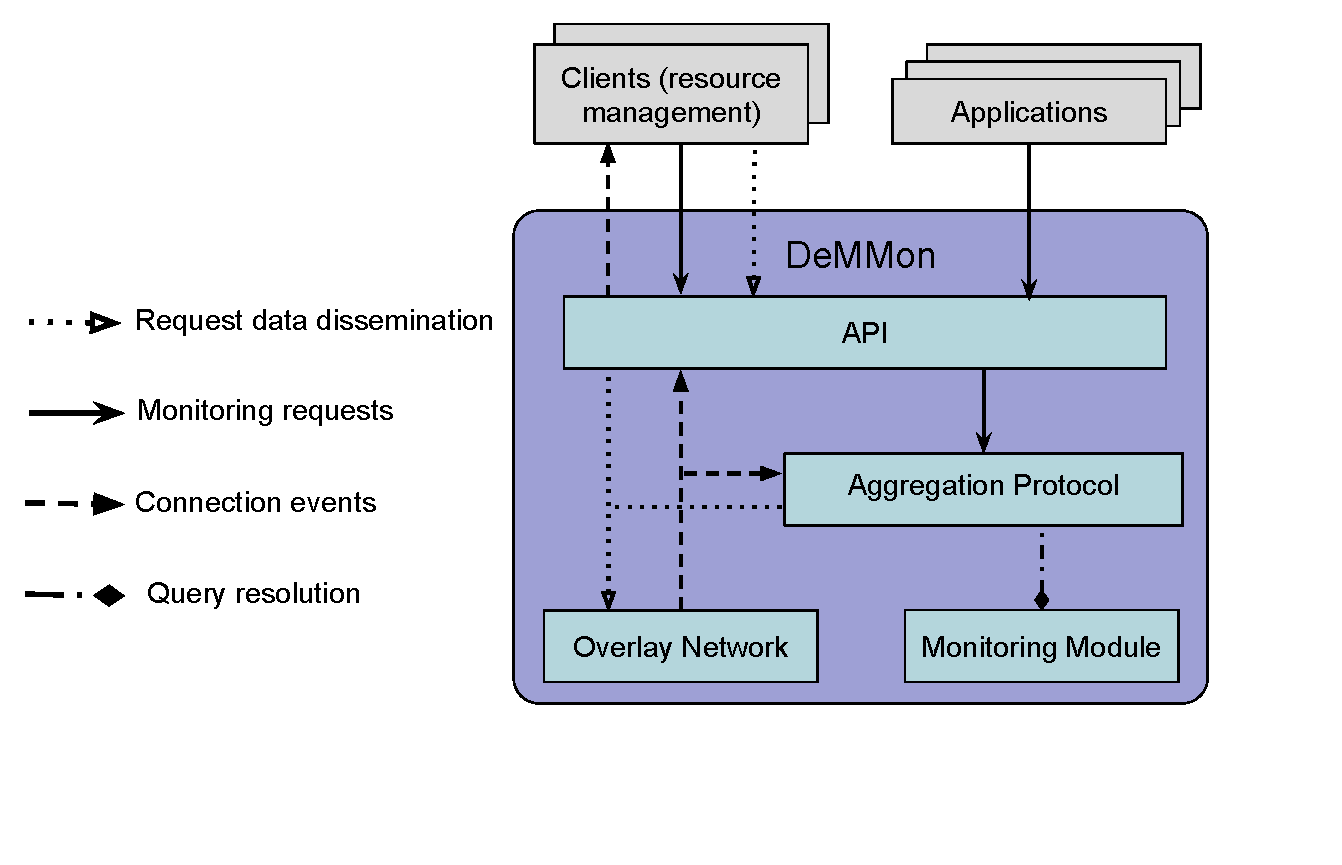
\includegraphics[width=\textwidth]{Chapters/Figures/DeMMon-overview.pdf}
    \caption{An overview of the architecture of DeMMon}
    \label{fig:demmon-overview}
\end{figure}
    
First, the \textbf{API} exposes the functionality of the framework, its main objectives are to (1) allow resource management solutions to collect metrics about nodes (or services they host) in the system; (2) allow those metrics to be queried through the use of a query language; (3) allow registering alarms which trigger based on conditions which evaluate the collected information. It is important to notice that the API is not the component tasked with gathering the information to perform these tasks. Instead, it exposes the results and mediates the interactions between the clients and the remaining modules.

Second, the \textbf{monitoring module} is tasked with storing metrics, resolving queries regarding stored metrics, removing expired metrics, periodically evaluating registered alarms, and triggering callbacks which the API then propagates to the client. This module satisfies points \ref{enum:demmon_4} and \ref{enum:demmon_6} of the aforementioned requirements.

The \textbf{overlay network} is responsible for building a latency-aware multi-tree-shaped network. Nodes in this network use latency, node capacity, and a set of logical rules to change their location either from one tree to another or within their tree until they have an optimized set of nodes (according to latency). The connections resulting from the operation of this protocol are the basis for the aggregation protocol. In addition, this module also offers limited horizon flood techniques, exposed through the API, fulfilling the points \ref{enum:demmon_1} and \ref{enum:demmon_5} of the requirements presented previously.

Finally, the \textbf{aggregation protocol} is a component that performs on-demand metric collection based on issued commands from the API. This component takes advantage of the overlay networks' established connections and hierarchical structure to perform efficient distributed aggregations. It allows three types of decentralized aggregation: (1) \textit{tree aggregation}, which consists of collecting metrics and merging them using the overlay protocols' trees, collecting a globally aggregated value in the tree roots (or a partial view of the system for nodes that are not the root of the overlay); (2) \textit{global aggregation}, where nodes also use their tree connections to efficiently collect a globally aggregated value (independently of being the root of the tree); and (3) \textit{neighbourhood aggregation}, where nodes collect values (non aggregated) of nearby nodes in term of hop proximity. These three mechanisms satisfy points \ref{enum:demmon_2}, \ref{enum:demmon_3} and \ref{enum:demmon_7} of the aforementioned requirements. 

In the following sections, we will provide a detailed explanation of each individual modules' design and implementation, starting by the \textbf{overlay network} (section \ref{sec:overlay_network}), followed by \textbf{aggregation protocol} (section \ref{sec:mon_protocol}), and lastly, the \textbf{monitoring module} (section \ref{sec:mon_module}) and \textbf{API} (section \ref{sec:api}). 

\section{Overlay network} 
\label{sec:overlay_network}


% Define tab size for indentation
\algrenewcommand\algorithmicindent{2em}%

%%%%%%%%%%%%%%%%%%%%%%%%%%%%%%%%%%%%%%%%%%%%%%%%%%%%%%%%%%%%%%%%
% BLOCKS - \block[]
%%%%%%%%%%%%%%%%%%%%%%%%%%%%%%%%%%%%%%%%%%%%%%%%%%%%%%%%%%%%%%%%

% State, like all blocks ends with \asdend
\algblockdefx[asdstate]{asdstate}{asdend}
{\textbf{State}}{}


% Init
\algblockdefx[asdinit]{asdinit}{asdend}
{\textbf{Init}}{}

\algblockdefx[asdtypes]{asdtypes}{asdend}
{\textbf{Types}}{}

\algdef{SE}[SUBALG]{Indent}{EndIndent}{}{\algorithmicend\ }%
\algtext*{Indent}
\algtext*{EndIndent}

% Upon
\algblockdefx[asdupon]{asdupon}{asdend}
[1][Unknown]{\textbf{Upon} #1 \textbf{Do}}{}
\algblockdefx[asdupontimer]{asdupontimer}{asdend}
[1][Unknown]{\textbf{Upon Timer} #1 \textbf{Do}}{}

% For
\algblockdefx[asdfor]{asdfor}{asdend}
[1][Unknown]{\textbf{Forall} #1 \textbf{Do}}{}

\algblockdefx[asdrepeateveryx]{asdrepeateveryx}{asdend}
[1]{\textbf{Every} #1 \textbf{Do}}{}

% If
\algblockdefx[asdif]{asdif}{asdend}
[1][Unknown]{\textbf{If} (#1) \textbf{Then}}{}

% Else for If
\algcblockdefx[asdelsea]{asdif}{asdelsea}{asdend}
{\textbf{Else}}{}

% Else for Else If
\algcblockdefx[asdelseb]{asdelseif}{asdelseb}{asdend}
{\textbf{Else}}{}

% Else If
\algcblockdefx[asdelseif]{asdif}{asdelseif}{asdend}
[1][Unknown]{\textbf{Else If} (#1) \textbf{Then}}{}

% Interface
\algblockdefx[asdinterface]{asdinterface}{asdend}
{\textbf{Interface}}{}

% Requests
\algblockdefx[asdrequests]{asdrequests}{asdend}
{\textbf{Requests}}{}

% Indications
\algblockdefx[asdindications]{asdindications}{asdend}
{\textbf{Indications}}{}

% Procedure
\algblockdefx[asdprocedure]{asdprocedure}{asdend}
[1][Unknown]{\textbf{Procedure} #1}{}

% Forever
\algblockdefx[asdforever]{asdforever}{asdend}
{\textbf{Forever Do}}{}

%%%%%%%%%%%%%%%%%%%%%%%%%%%%%%%%%%%%%%%%%%%%%%%%%%%%%%%%%%%%%%%%
% STATEMENTS - \statement{} or \statement{}{}
%%%%%%%%%%%%%%%%%%%%%%%%%%%%%%%%%%%%%%%%%%%%%%%%%%%%%%%%%%%%%%%%

% Simple Statements
\newcommand{\asdstatement}[1]{\statenew{#1}}
\newcommand{\asdstatementbold}[1]{\statenew{\textbf{#1}}}

% Trigger
\newcommand{\asdtrigger}[1]{\statenew{\textbf{Trigger} #1}}

% Timer
\newcommand{\asdsetuptimer}[1]{\statenew{\textbf{Setup Timer} #1}}
\newcommand{\asdsetupptimer}[1]{\statenew{\textbf{Setup Periodic Timer} #1}}
\newcommand{\asdcanceltimer}[1]{\statenew{\textbf{Cancel Timer} #1}}

% Call
\newcommand{\asdcall}[1]{\statenew{\textbf{Call} #1}}

% Return - use [] due to xparse
\NewDocumentCommand{\asdreturn}{o}{
	\statenew{\textbf{Return}\IfValueT{#1}{ #1}}
}

% Comment (inline)
\makeatletter
\newcommand{\asdcomment}[1]{
	\parbox[t]{\dimexpr\linewidth-\ALG@thistlm-8em}{
		\strut
		//\space #1
		\strut
	}
}
\makeatother


% Comment (entire line)
\makeatletter
\newcommand{\asdlinecomment}[1]{
		\State \parbox[]{\dimexpr\textwidth-\leftmargin-\labelsep-\labelwidth}{
			//\space #1
		\strut}
}
\makeatother


%%%%%%%%%%%%%%%%%%%%%%%%%%%%%%%%%%%%%%%%%%%%%%%%%%%%%%%%%%%%%%%%
% VALUES
%%%%%%%%%%%%%%%%%%%%%%%%%%%%%%%%%%%%%%%%%%%%%%%%%%%%%%%%%%%%%%%%

% Booleans
\newcommand{\asdfalse}[0]{$false$}
\newcommand{\asdtrue}[0]{$true$}

% Map
\newcommand{\asdmap}[2]{#1{[}#2{]}}

% Set 
\newcommand{\asdset}[1]{$\{$#1$\}$}

%%%%%%%%%%%%%%%%%%%%%%%%%%%%%%%%%%%%%%%%%%%%%%%%%%%%%%%%%%%%%%%%
% Algebraic
%%%%%%%%%%%%%%%%%%%%%%%%%%%%%%%%%%%%%%%%%%%%%%%%%%%%%%%%%%%%%%%%

% Equals (assignment)
\newcommand{\asdassign}[0]{ $\longleftarrow$ }

\algblockdefx[Foreach]{Foreach}{EndForeach}[1]{\For{\textbf{each} #1}}{}

% Equals (comparison)
\newcommand{\asdeq}[2]{#1 $=$ #2}

% Not equals
\newcommand{\asdneq}[2]{#1 $\neq$ #2}

% Exists
\newcommand{\asdexists}[1]{$\exists$ #1}

% Not Exists
\newcommand{\asdnexists}[1]{$\nexists$ #1}

% And
\newcommand{\asdand}[2]{#1 $\wedge$ #2}

% Or
\newcommand{\asdor}[2]{#1 $\vee$ #2}

% Except
\newcommand{\asdexcept}[2]{#1 $\setminus$ #2}

% Union
\newcommand{\asdunion}[2]{#1 $\bigcup$ #2}

% Belongs to
\newcommand{\asdin}[2]{#1 $\in$ #2}

% Not belongs to
\newcommand{\asdnotin}[2]{#1 $\notin$ #2}

% Bottom
\newcommand{\asdbottom}{$ \perp $}

\algnewcommand{\IfThenElse}[3]{% \IfThenElse{<if>}{<then>}{<else>}
  \State \algorithmicif\ #1\ \algorithmicthen\ #2\ \State \algorithmicelse\ #3}


%%%%%%%%%%%%%%%%%%%%%%%%%%%%%%%%%%%%%%%%%%%%%%%%%%%%%%%%%%%%%%%%
% Other
%%%%%%%%%%%%%%%%%%%%%%%%%%%%%%%%%%%%%%%%%%%%%%%%%%%%%%%%%%%%%%%%

\newcommand{\asdnewline}{\hfill\State}

In this section, we discuss the design of the devised overlay network protocol, which aims to build and maintain a latency and capacity-aware tree-shaped network , where capacity represents one, or a combination of, values that denote the node's networking or computing capacity (in our case, we used only bandwidth as each nodes' capacity). We begin by providing the considered system model, then follow with an overview of the mechanisms responsible for building and maintaining the tree, and lastly, we conclude the chapter with a summary and discussion of the protocol.

\subsection{System Model}

The intended system model for this protocol is a distributed scenario composed of nodes connected to the internet and set up to enable the reception or emission of messages via the internet (either with an external IP or port-forwarding). We also assume that nodes are spread throughout a large area, have varied capacity values, and are distributed among both Cloud and Edge settings.

Regarding the fault model, we assume that all but a small portion of nodes (also known as the landmarks, which in our model represent data centres) can fail, and when other nodes fail, they do so in a crash-fault manner, stopping the execution of the process along with all emissions and receptions of messages at the time of failure. We assume landmarks have additional fault tolerance provided their privileged infrastructure, or alternatively, we assume that other mechanisms such as replication could be employed to ensure that faulty landmarks are swiftly replaced in place in case of failure. 
  
Finally, all nodes must run the same software stack with similar configuration settings, installed a priori.

\subsection{Overview}

As previously mentioned, the main objective of the devised protocol is to establish a latency and capacity-aware multi-tree-shaped overlay network, rooted on the previously mentioned landmarks. The motivations for the choice of a tree structure for our network are the following: (1) to map the cloud-edge environment, by rooting the trees on nodes running DCs in the cloud, and setting up the remaining nodes with less capacity in positions where they can be coordinated from the roots (2) to be able to map the heterogeneity of each device in the environment: by biasing the placement of nodes in the tree such that nodes with higher capacity are placed higher in the tree, and nodes with lower capacity are biased towards lower levels of the tree, nodes are used more or less according to their capacity values; (3) the tree structure can be easily employed to perform efficient aggregations, by propagating and merging values recursively from the lower to the higher levels of the tree, which is the basis for the aggregation protocol presented in \ref{sec:mon_protocol:tree_agg}; and finally, (4) by leveraging on the tree structure, nodes can propagate information efficiently, given that, in a network composed of N nodes, broadcasts require only N-1 message transmissions to reach all nodes in the network. 

\begin{figure}[htbp]
    \centering
    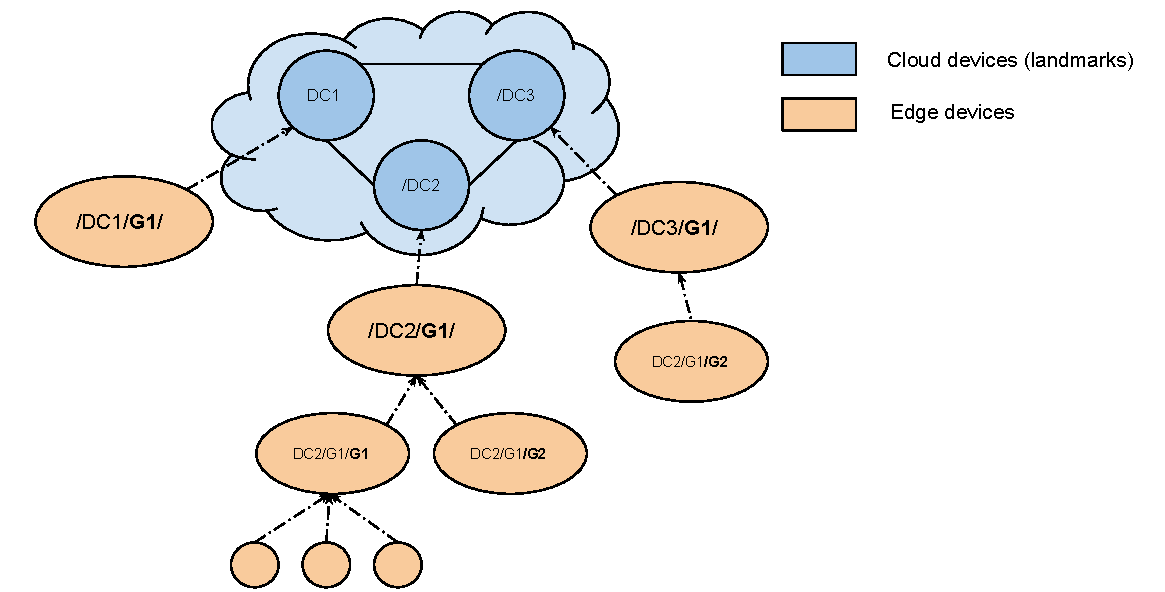
\includegraphics[width=\textwidth]{Chapters/membership/images/DeMMon-overlay-structure.pdf}
    \caption{An example of a network established by the devised protocol (with 3 landmarks)}
    \label{fig:demmon-membership-structure}
\end{figure}

The type of tree structure our protocol aims to establish and maintain is observable in figure \ref{fig:demmon-membership-structure}, which, as previously referenced, is composed of multiple interconnected trees. As observable, every node is attributed an identifier, which is the concatenation of the parents' ID with an assigned ID (this mechanism is explained in further detail in subsection \ref{sec:overlay_network:oportunistic_improvement}). The nodes connected to the landmarks (denoted their \textbf{children}) may themselves be the \textbf{parent} of their own children, which would have the landmark as their \textbf{grandparent} (which is the case of ``/DC2/G1/G2'' and ``/DC2/G1/G1''). Intuitively, the \textbf{descendants} of a node are all of its children and children's children, recursively, until the leaves. All nodes which share the same parent (\textbf{siblings}) are connected among themselves, forming a \textbf{group}, whose size is biased (but not guaranteed) to be within two configurable upper and lower bounds. Therefore, all nodes have active connections to their parent, children and siblings. The combination of a node's active connections may be called its \textbf{active view}. 

The devised algorithm is composed of three main mechanisms: (1) the \textbf{join} mechanism, which aims to establish the initial tree structures, (2) the \textbf{active view maintenance}, responsible for biasing the number of connections for each node and optimizing the connections of each node, (3)  and finally \textbf{passive view maintenance}, responsible for collecting information about peers which are not in the active view, which are used for both fault tolerance and connection optimizations.

\subsubsection{Join mechanism} \label{sec:overlay_network:join}

The Join mechanism is the mechanism responsible for establishing an initial parent connection. It is the aim of this mechanism (from the joining node standpoint), to establish a connection with the node with the least cost possible. This mechanism is the first to be executed by all nodes in the system, and it essentially consists in a depth-first search in the established DeMMon trees. The pseudocode for this algorithm can be observed in \ref{alg:memb:join}. 

% JOIN -----

\begin{algorithm}{}
\caption{Join Protocol} \label{alg:memb:join}
% \setstretch{0.85}
\begin{algorithmic}[1]
    \asdtypes
        \State Node : <lat, parentIP, nrChildren, replied, IP, ID, coords, version, children<IP,  nrChildren\>\>
    \asdend
    \asdstate \label{alg:memb:join:state}
        \State contactedNodes \Comment{collection of all successfully contacted nodes}
        \State nodesToContact set<Node> \Comment{nodes being contacted}
        \State joinTimeouts : dict<Node, time> \Comment{collection of contacted nodes -> timerIDs}
        \State bestPeerLastLevel : Node \Comment{the best peer contacted so far in the join process}
        \State joinReqTimeoutTid : string \Comment{ timerID for join messages}
        \State prevBestP : Node \Comment{ myself}
        \State landmarks : set<IP> \Comment{landmark nodes}
    \asdend

\asdupon[Init(landmarks : set<IP>, selfIP, isLandmark)] \label{alg:memb:join:init}
    \State landmarks \asdassign landmarks 
    \State joinTimeouts, prevBestP \asdassign \{\}, nil
    \IfThenElse{isLandmark}
    {addLandmarkUntilSuccess(landmarks) \label{alg:memb:join:add_land}} 
    {contactNodes(landmarks) \label{alg:memb:join:contact_landm}} 
\asdend


\asdupon[receive(Join<>,sender)] \label{alg:memb:join:recv_join}
    \State sendMessageSideChannel(JoinReply<self.parent, self.node, self.children>, sender) 
\asdend
    
\asdupon[receive JoinReply(<parentIP, node, children>, sender) \&\& measuredLatency(lat)]  \label{alg:memb:join:recv_join_reply}
        \If{\asdin{node.IP}{nodesToContact}} 
            \If{\asdin{parentIP}{Landmarks}}
                \State self.coordinates[getIdx(landmarks, sender)] = lat
            \EndIf
            \State nodesToContact[node.IP].lat \asdassign lat
            \State nodesToContact[node.IP].children \asdassign children
            \State nodesToContact[node.IP].parent \asdassign parentIP
            \State nodesToContact[node.IP].replied \asdassign true
            \State cancelTimer(joinTimeouts[sender])
            \State delete(joinTimeouts, sender)
        \Else
            \State nodesToContact.delete(node)
        \EndIf
\asdend

\asdupon[(forall n $\in$ nodesToContact -> n.replied)] \label{alg:memb:join:cond_go}
    \State contactedNodes.appendAll(nodesToContact)
    \For{node in sortedByLatency(nodesToContact)}
        \If{(\asdnotin{node.IP}{landmarks}) \&\& node.nrChildren == 0} \label{alg:memb:join:verif_children}
            \State continue \Comment{check if node has enough children}
        \EndIf
        \If{prevBestP != nil \&\& (prevBestP.lat $\le$ node.lat || prevBestP.nrChildren < config.minGroupSize)} \label{alg:memb:join:verif_vs_prev}
            \State joinAsChild(prevBestP)
        \Else
            \State prevBestP \asdassign node \label{alg:memb:join:advance}
            \State toContact \asdassign [\asdin{c}{prevBestP.children} -> c.nrChildren > 0]
            \State contactNodes([c.IP for c in toContact])
        \EndIf
        \State return
    \EndFor
    \IfThenElse{prevBestP != nil} 
    {joinAsChild(prevBestP)}  \label{alg:memb:join:join_base_case}
    {abortJoinAndRetryLater()} 
    \State return
\asdend

\asdupon[JoinTimeoutTimer(node) || NodeMeasuringFailed(node)] \label{alg:memb:join:exclusions}
    \IfThenElse{(L in Landmarks)}{abortJoinAndRetryLater()}{delete(nodesToContact[L])} 
\asdend

\asdupon[JoinRequestTimer(p : Node)]
    \If {sender == prevBestP}
        \If{p.parentIP != nil}
            \State prevBestP \asdassign contactedNodes[p.parentIP]
            \State joinAsChild(prevBestP)
        \Else
            \State abortJoinAndRetryLater()
        \EndIf
    \EndIf
\asdend

\asdupon[receive(JoinRequest<>, sender)]
    \State childID \asdassign addChildren(sender) \Comment{new chilren is established, and an ID is generated for it}
    \State sendMessageSideChannel(JoinRequestReply<childID, self>, sender)
\asdend
    
\asdupon[receive(JoinRequestReply<myID, parent>, sender)]
    \If {sender == prevBestP} 
        \State parent \asdassign sender \Comment{Adds Parent is established, join complete}
        \State cancelTimer(joinReqTimeoutTid)
        \State self.ID \asdassign parent.ID + "/" + myID \Comment{Later used in shuffle mechanism}
    \EndIf
\asdend

\asdprocedure[joinAsChild(p : Node)]
    \State joinReqTimeoutTid \asdassign setupTimer(JoinRequestTimer<p>, config.JoinTimeout)
    \State sendMessageSideChannel(JoinRequest<>, p.IP)
\asdend

\asdprocedure[contactNodes(ips : IP{[]})]
    \State nodesToContact \asdassign \{\}
    \State toContact \asdassign [Node<0,nil,0,false,ip,false,[]> for ip in ips]
    \For{n in toContact}
        \State nodesToContact[n] \asdassign n
        \State MeasureNode(n) 
        \State sendMessageSideChannel(JoinMessage<>, n)
        \State joinTimeouts[n] \asdassign \asdassign setupTimer(JoinTimeoutTimer(n), config.JoinTimeout)
    \EndFor
\asdend

\end{algorithmic}
\end{algorithm}


The first step of the algorithm (line \ref{alg:memb:join:state}) is to initialize the state of the joining node, that is materialized by: (1) a map called ``contactedNodes'' of type ``Node'', containing all nodes contacted successfully in the join process (indexed by a string representation of their IP), (2) a collection named ``nodesToContact'' of type ``Node'' containing the nodes to yet to contact in the join process, (3) a map of timer IDS indexed by strings, containing the timer IDS for each contacted node, named ``joinTimeouts'', (4) a variable called ``bestPeerLastLevel'' containing the best (lowest latency) node contacted so far in the join process, (5) a variable named ``joinReTimeoutId'', containing a timer id for a timer used as a timeout for the chosen node in the join process, (6) a variable of type ``Node'' denoting the peer executing the protocol, and finally (7), a set containing the landmarks of the network, named ``landmarks''. The type ``Node'' is a collection of attributes regarding a certain physical node, composed of: (1) latency measured, (2) its current parent, (3) number of children, (4) whether the node replied to the message, (5) its IP, (6) an array of coordinates (denoting its measured latency to each landmark, used in passive view maintenance mechanism), and finally, (7) an array of its childrens' IP and their respective number of children.
 
The procedures taken to join the tree differ consonant the node is a landmark or not. In the case of landmarks, these attempt to repeatedly establish a connection with other landmarks through the emission of a special message. Landmarks that receive this message always send a reply and establish a connection to the sende of the message (line \ref{alg:memb:join:add_land}). Any joining landmark only stops sending messages to other landmarks when the respective reply is received, and an outgoing connection is established.

Nodes that are not landmarks begin the process of finding their initial parent in the DeMMon tree. This process is initiated by measuring the current latency and sending a JOIN message (via a temporary TCP channel) to the landmarks. For each message sent, a timer is created, and its ID is stored in the ``joinTimeouts'' map (line \ref{alg:memb:join:contact_landm}). Whenever a node receives this JOIN message, it sends a JOINREPLY message back to the original sender containing: its parent, itself, and its children (line \ref{alg:memb:join:recv_join}).

During the wait process, the joining node waits for either the responses from the contacted nodes, for any timer in the ``joinTimeouts'' map to trigger, or for any failed latency measurements. In the second and third case, the contacted node is excluded from the join process, and it is resumed as normal (line \ref{alg:memb:join:exclusions}). In case there are no nodes left to resume the join process or if the excluded node is a landmark, then the node waits a configurable amount of time until attempting to re-join the overlay again. 

If the contacted node has not failed, and the joining node receives the JOINREPLY (line \ref{alg:memb:join:recv_join_reply}), it checks if it came from a timed-out node or from any node whose parent was not contacted in the join process (e.g. if the contacted node changed parent during the join process), if any of these situations occurs, then the message is discarded. If none of these situations occurs, the message is not discarded, and the information contained in the JOINREPLY message is stored in the ``contactedNodes'' map.

Whenever the joining node has either received the JOINREPLY messages from all contacted nodes or they have been excluded from the join process, it evaluates all the successfully contacted nodes attempting to find the contacted node with the lowest latency which is a suitable parent. This procedure is performed by sorting the nodes in ascending order of measured latency and performing the following verifications:

\begin{enumerate}
    \item Verify that the node  Verify if the node already has any children or if the node is a landmark (landmarks can become parents of any node, except other landmarks) (line \ref{alg:memb:join:verif_children}). 
    
    \item Verify if there was a node already contacted previously which was a suitable parent and had lower measured latency. In case there was, the joining node sends a ``JoinRequest'' message (requesting to be its child), sets up a ``JoinRequestTimer'' for that node, and stops the verification process. (line \ref{alg:memb:join:verif_vs_prev})

    \item Verify if the current node has both enough children, and has the lowest latency up to this point in the join process, then the joining node assigns it as its best node so far and starts a new recursive step by sending JOIN messages and measuring the children of that node which themselves have more than one children (line \ref{alg:memb:join:advance}). Note that if none the current nodes' children are suitable parents (i.e. have no children themselves), then the condition in line \ref{alg:memb:join:cond_go} is triggered and the joining node will request the current best node to be its parent.
\end{enumerate}

If none of the verified peers was suitable to start a new recursive step (if they either had no children or all verified nodes had higher latency than a previously contacted node), (line \ref{alg:memb:join:join_base_case}), then the node joining node sends a ``JoinRequest'' to that node and sets up a ``JoinRequestTimer'' for the best previously contacted node (any node which receives a ``JoinRequest'' message replies with a ``JoinRequestReply''). 

The join process is concluded with both the reception of a ``JoinRequestReply'' and the establishment of the connection between the sender and receiver of the message. If the ``JoinRequestTimer'' timer triggers while waiting for the response, the node will fall back to the parent of the selected node (and do so recursively, in case the parent failed aswell) or re-join the overlay later in case there is no parent available. 

\subsubsection{Active view maintenance} \label{sec:overlay_network:active_view_maint}

The second mechanism of the devised membership algorithm, called active view maintenance, is the mechanism responsible for maintaining the size of the groups. In sum, this mechanism is coordinated by each parent and achieved via sending messages to some of its children signalling that they should connect to another specified parent. It achieves this by choosing new parents to form new groups using latency and node capacity as heuristics for the parent choice, where the information necessary to employ these two heuristics is obtained via periodic transmission from every child to its parent. This mechanism only executes when a group exceeds its size limit and attempts to keep group sized near the maximum configured limit.

The pseudocode for this mechanism is presentend in algorithm \ref{alg:memb:active_view_maint}, and starts by defining the necessary state: the nodes' active view (parent, children, and siblings), and an auxiliary map of sets, which holds the latencies of each children to every other children. (lines \ref{alg:memb:active_view_maint:state_start}-\ref{alg:memb:active_view_maint:state_end}). 

\begin{algorithm}
    \caption{Membership protocol (Active view Optimization)} \label{alg:memb:active_view_maint}
    % \begin{multicols}{2}
    % \setstretch{0.85}
    \begin{algorithmic}[1]
        \asdstate
            \State parent \Comment{defined in join} \label{alg:memb:active_view_maint:state_start}
            \State children \Comment{defined in join} 
            \State siblings  
            \State childrenLatencies : dict<string:dict<string:number>> \label{alg:memb:active_view_maint:state_end} \Comment{Holds the latencies of each children to every other children}
        \asdend

        \asdrepeateveryx{config.updatePeriodicity} \label{alg:memb:active_view_maint:update}
            \If{parent != nil}
                \State sLatencies \asdassign set()
                \For{sibling in siblings}
                    \State sLatencies.append(<sibling.IP,sibling.measuredLatency)
                \EndFor
                \State sendMessage(UpdateChildStatus<children, siblingLatencies>, parent)
            \EndIf
            \For{child in chidren}
                \State sendMessage(UpdateParentStatus<self, chidren \\ child>)
            \EndFor
        \asdend \label{alg:memb:active_view_maint:update_end}

        \asdupon[receive(UpdateParentStatus<parent, children>, sender)] 
        \label{alg:memb:active_view_maint:update_recv_par}
            \If{sender == parent.IP}
                \State parent \asdassign parent
                \State self.ID \asdassign parent.ID + "/" + myID
                \State grandParent \asdassign grandParent
                \State siblings \asdassign siblings
                \State measureSiblingLatency(siblings)
            \EndIf
        \asdend

        \asdupon[receive(UpdateChildStatus<child, childSiblingLatencies>, sender)]\label{alg:memb:active_view_maint:update_recv_chi}
            \If{children[sender] != nil}
                \State children[sender]\asdassign child
                \State childrenLatencies[sender] \asdassign childSiblingLatencies
            \EndIf
        \asdend
    
    % \end{algorithmic}
    % \columnbreak
    % \begin{algorithmic}
    
        \asdrepeateveryx{config.evalGroupSize} \label{alg:memb:active_view_maint:update_eval}
            \If{len(children) <= config.maxGroupSize}
                \State return
            \EndIf
            \State childrenLatValues \asdassign set()
            \For{c1 in children} \label{alg:memb:active_view_maint:update_eval_merge_start}
                \For{<c2, lat> in childrenLatencies[c]}
                    \If{lat - c1.measuredLatency > d.config.maxLatDowngrade}
                        \State continue
                    \EndIf
                    \IfThenElse{c1.cap > c2.cap}
                    {childrenLatValues.add(<c1,c2,lat>)}
                    {childrenLatValues.add(<c2,c1,lat>)}
                \EndFor
            \EndFor \label{alg:memb:active_view_maint:update_eval_merge_finish}
            \State kickedNodes, newParents \asdassign set(),set()
            \State pChildren \asdassign dict<string,set<Node{>}{>} \Comment{set of potential children for each children}
            \State sortByLatency(childrenLatValues)
            \State idealGroupSize \asdassign config.maxSize - config.MinGroupSize
            \For{<c1,c2,lat> in childrenLatValues}
                \If{len(children) - len(kickedNodes) <= config.maxSize} \label{alg:memb:active_view_maint:check_done_1}
                    \State break
                \EndIf
                \If{\asdin{c1}{kickedNodes} || \asdin{c2}{kickedNodes} ||  \asdin{c1}{newParents}} \label{alg:memb:active_view_maint:check_done_2}
                    \State continue
                \EndIf
                \If{c1.nrChildren == 0 \&\& newParents[c1] == nil} \Comment{Node is not yet a parent}
                    \State pChildren[c1] \asdassign pChildren[c1] + c2 \label{alg:memb:active_view_maint:add_set}
                    \If{len(pChildren) == config.MinGroupSize}
                        \For{potentialChild in pChildren[c1]} \label{alg:memb:active_view_maint:kick_set_start}
                            \State newParents \asdassign newParents + c1
                            \State kickedNodes \asdassign kickedNodes + potentialChild
                            \State send(OptimizationPropose<c1>, potentialChild)
                        \EndFor
                        \For{<nIP,pontentialChildrenTmp> in pChildren}
                            \State pontentialChildrenTmp.deleteAll(pChildren[c1])
                        \EndFor
                        \State pChildren[c1] \asdassign set<Node> \label{alg:memb:active_view_maint:kick_set_end}
                    \EndIf
                \Else \label{alg:memb:active_view_maint:kick_already_parent}
                    \State kickedNodes \asdassign kickedNodes + c2
                    \State send(OptimizationPropose<higherCapNode>, lowerCapNode)
                \EndIf    
            \EndFor
        \asdend

        \asdupon[receive(OptimizationPropose<newParent>, sender)] \label{alg:memb:active_view_maint:opt_propose_recv}
            \If{sender == parent}
                \State send(OptimizationProposeRequest<sender>, newParent)
            \EndIf
        \asdend

        \asdupon[receive(OptimizationProposeRequest<p>, sender)] \label{alg:memb:active_view_maint:opt_propose_req_recv}
            \If{ p == parent \&\& sender in siblings} \Comment{ parent issuing the message is my parent}
                \State addChild(sender)
                \State send(OptimizationProposeRequestReply<true,p>, sender)
            \Else
                \State sendSideChannel(OptimizationProposeRequestReply<false,p>, sender)
            \EndIf
        \asdend

        \asdupon[receive(OptimizationProposeRequestReply<reply,p>, sender)] \label{alg:memb:active_view_maint:opt_propose_req_reply_recv}
            \If{parent == p}
                \If{reply}
                    \State sendMessageAndDisconnectFrom(DisconnectMessage<>, parent)
                    \State addParent(sender)
                \EndIf
            \Else
                \State sendMessageTemporaryConn(DisconnectMessage<>, p)
            \EndIf
        \asdend

    \end{algorithmic}
% \end{multicols}
\end{algorithm}

The mechanism starts with the propagation of information from the parent to the children and vice-versa. As observable in lines \ref{alg:memb:active_view_maint:update}-\ref{alg:memb:active_view_maint:update_end}), each parent transmits to its children a list of its current siblings, and propagates to its parent the latency to each of its siblings. Then, when this information is received (lines \ref{alg:memb:active_view_maint:update_recv_par} and \ref{alg:memb:active_view_maint:update_recv_chi}), it is merged into their local states for later use.

The second part of this mechanism is also periodic and is responsible for maintaining the group sizes by creating new parents or by sending children to already created groups (line \ref{alg:memb:active_view_maint:update_eval}). This mechanism is only executed if the number of children of a certain node (denoted the ``proposer'') exceeds the configured maximum number of children per parent. In this mechanism, a proposer node proposes to one of its children (denoted node ``A'') a change of parent to another one of its children, (denoted the ``proposed'' node).


When triggered, the proposer node begins by merging all of its received latency pairs into a single set, where the node with the highest capacity is the first node of each pair. While doing so, it discards any new edges which would otherwise lower the overall latency of the system by a larger than configured amount (lines \ref{alg:memb:active_view_maint:update_eval_merge_start}-\ref{alg:memb:active_view_maint:update_eval_merge_finish}). Then, the node iterates the added edges set by ascending order of latency, performing the following verifications:

\begin{enumerate}
    \item If the number of current children minus the nodes already sent to a lower level is lower than the maximum size of a group, then the node concludes the mechanism (line \ref{alg:memb:active_view_maint:check_done_1})
    
    \item If any of the two nodes were already sent to lower levels of the tree, then the current edge is skipped (line \ref{alg:memb:active_view_maint:check_done_2}).
    
    \item Then, if the node with higher capacity of the edge pair has no children yet, the lower capacity node is added to its ``possibleChildren'' set (line \ref{alg:memb:active_view_maint:add_set}). When this set has the same size as the minimum configured group size, then the node issues ``OptimizationPropose'' messages for each node of the set, and removes each child from every other node's potential children (lines \ref{alg:memb:active_view_maint:kick_set_start}-\ref{alg:memb:active_view_maint:kick_set_end}). Alternatively, if the higher capacity node already is a parent (either because some nodes were already chosen to form its group, or because it was already a parent previously), then the coordinator node issues a ``OptimizationPropose'' message to it (line\ref{alg:memb:active_view_maint:kick_already_parent}).
\end{enumerate}

When node ``A'' receives an ``OptimizationPropose'' message with a new proposed parent (line \ref{alg:memb:active_view_maint:opt_propose_recv}), it verifies that the message was sent by its current parent, discarding it if it is not. After this, it sends an ``OptimizationProposeRequest'' message containing itself and the proposer node to the proposed parent, signalling it wishes to become its child. Then, when the proposed parent receives the message (line \ref{alg:memb:active_view_maint:opt_propose_req_recv}), it verifies that the proposer node is still its parent and that node ``A'' is also its sibling, if yes, then it adds the node as its new child and replies with an ``OptimizationProposeRequestReply'', which contains a boolean flag, signalling if the node was added as a child or not. Lastly, when this message is received (line \ref{alg:memb:active_view_maint:opt_propose_req_reply_recv}), the node also verifies that the proposer node is still its parent, aborting the process if it is not, and adds the proposed node as its parent.

After this process is complete, if not aborted, the proposed node becomes the parent of node ``A'', and the proposer node has fewer children, reducing its group size towards the configured maximum (as the proposer node only executes this mechanism if its children number exceeds the configured amount), and when possible, node ``A'' obtains a new node with lower latency than its current latency to the proposer node.

It is important to note that since the mechanism limits the latency downgrade for each new parenthood connection, it does not guarantee that the group sizes are bounded. Although it would be possible to bound the number of nodes per group if this condition were ignored, then the mechanism would conflict with the third mechanism, which we will explain further in the document. \todo{ref to code}

It is important to mention a final mechanism in active maintenance which is ommited from the pseudocode. This mechanism is responsible for ensuring that groups sizes do not become too small, according to a configuration parameter. In sum, every node periodically verifies the number of peers which are its siblings, if this number is lower than a certain threshold, the node ``rolls a dice'' (essentially generates a random number and verifies if it is lower than a certain threshold) to decide if it should abandon the current group. If the generated number is lower than the threshold, the node sends a message to its grandparent asking to become its child. When the grandparent receives the message, it adds the node to its children and sends a message reply, signalling to the original node that it was accepted as a child. It is important to mention that the aforementioned threshold of the ``dice roll'' (and consequently the probability of the node remaining in the current group) decreases quadratically to the difference of the configured group size and the current node's group size.

\subsubsection{Passive view maintenance \& Oportunistic improvement} \label{sec:overlay_network:oportunistic_improvement}

The third mechanism of the devised membership algorithm is the passive view maintenance mechanism, it is responsible for creating an auxiliary pool of nodes in the overlay which are not descendants of the executing node. When full, the pool serves two purposes: the first is to enable fault tolerance in the overlay without having to rely on the landmarks, the second is to enable the self-improvement of the overlay. 

There are three components of the Node type (the ID, Coordinates and the version of each node) which were present in the pseudocode of the previous mechanisms, but their explanation was omitted given they are only relevant to the behaviour of the following mechanism. We now explain each in detail, and how it is obtained:

\begin{enumerate}
    \item The ID of each node is a collection of ID segments, where each node's ID is the concatenation of every segment of every ascendant of the node with its own segment. Each node's segment is generated by each parent whenever a new node requests to be its child. An example of a possible ID would be: AAA/BBB/CCC, where the ID segments are: ``AAA'' ,``BBB'' and ``CCC'', this gives each node enough information based on an ID to evaluate if any other node in the overlay is its a descendent, therefore allowing nodes to evaluate if a change of parent in the overlay causes a cycle in the tree. This ID structure also allows nodes check what is the level of any node (the number of segments of the ID is the same as the level of a node in the tree).
    
    \item The coordinates are an array of integers representing the latency every node measured to all landmarks, these coordinates are used as a heuristic for measuring new nodes in the passive view which are potential parents.
    
    \item The version of a node is a monotonic integer which is incremented at every ID change and child addition or removal. This version is used in random walks, to update peers which are currently in the passive view with their new IDs, which prevents nodes from attempting to measure nodes which would be incompatible parents (i.e. they are their descendants, or have no children themselves)
\end{enumerate}

With these concepts explained, we now present the pseudocode (algorithm \ref{alg:memb:passive_view_maint}) for the mechanism. The first lines declare the new necessary state to the mechanism, which is composed of a set of nodes denoting the passive view of the node (line \ref{alg:memb:passive_view_maint:state}). Then, in the following lines we may observe the mechanism for filling the passive view, this is a periodic procedure which triggers the emmision of new random walk messages, triggered at pre-configured intervals (line \ref{alg:memb:passive_view_maint:walk_trig}), the created random walk message contains a random sample of nodes from the passive view and the active view, the original sender's ID, and an integer representing the messages' time-to-live (TTL). This message is then sent to a node that is not a descendant of the sender.

\begin{algorithm}
\caption{Membership protocol (Oportunistic Optimization)}
\begin{algorithmic}[1]
    

    \asdstate
        \State eView : set<Node>
    \asdend

    \asdrepeateveryx{config.RandWalkPeriodicity}
        \State ascNeighs, allNeighs = set
        \State ascNeighs = ascNeighs + parent + siblings
        \State allNeighs = allNeighs + ascNeighs + children
        \State sample = getRandSample(eView + allNeighs, config.NrPeersToMergeRandWalk)
        \State sendMessage(RandomWalk<sample, config.RandWalkTTL, self.ID, self.IP>, getRand(ascNeighs))
    \asdend

    \asdrepeateveryx{config.OportunisticOptimizationTimeout}
        \State toMeasureRand = getRandSample(eView, config.NrPeersToMeasureRandom)
        \State toMeasureBiasedOpts = sortByEuclideanDist(eView / toMeasureRand)
        \State toMeasureBiased = getRandSample(toMeasureBiasedOpts, config.NrPeersToMeasureRandom)
        \For p in toMeasureRand:
            \State measurePeer(p)
        \EndFor
        \For p in toMeasureBiased:
            \State measurePeer(p)
        \EndFor
    \asdend


    \asdupon[receive( RandomWalk<sample, ttl, nID, orig>, sender)]
        \State stepsTaken = config.RandWalkTTL - ttl
        \State nrToAdd = config.NrPeersToMergeRandWalk
        \State nrToMerge = config.NrPeersToMergeRandWalk
        \State ascNeighs, allNeighs = set(), set()
        \State ascNeighs = ascNeighs + parent + siblings
        \State allNeighs = allNeighs + ascNeighs + children

        \If{stepsTaken < config.NrStepsToIgnore}:
            \State nrToMerge = 0
        \EndIf

        \State toAdd = getRandSample(excludeDescendantsOf([eView + allNeighs] / sample),nID), nrToAdd)
        \State toRemoveFromSample = getRandSample(sample, nrToMerge)
        \State sample = sample / toRemoveFromSample
        \State sample = sample + toAdd
        \State target = getRand(excludeDescendantsOf(allNeighs, nID)
        \If{target == nil || ttl == 0}
            \State sendMessageSideChannel(RandomWalkReply<sample>, orig)
        \Else
            \State sendMessage(RandomWalk<sample, ttl-1, nID, orig>, getRandom(ascNeighs))
        \EndIf
        \State eView = excludeDescendantsOf(toRemoveFromSample, self.ID)  + eView
        \State eView = eView / allNeighs
        \State eView = eView[:config.MaxEViewSize]
    \asdend

    \asdupon[peerMeasured(p, latency)]
        \State latencyImprovement := parent.measuredLatency - Latency
        \If{latencyImprovement >= config.MinLatencyForImprovement}
            \State sendMessageSideChannel(OportunisticImprovementReq<self>,p)
        \EndIf
    \asdend


    \asdupon[receive(OportunisticImprovementReq<p>,sender)]
        \If{isDescendent(p.ID,self) or parent == nil}
            \State sendMessageSideChannel(OportunisticImprovementReqReply<false>,sender)
        \Else
            \State addChildren(sender)
            \State sendMessageSideChannel(OportunisticImprovementReqReply<true>,sender)
        \EndIf
    \asdend

    \asdupon[receive(OportunisticImprovementReqReply<answer>,sender)]
        \If {answer} 
            \State addParent(sender)
        \EndIf
    \asdend

    \asdprocedure[isDescendentOf(nodeID, PotentialDescID)]
        \State return PotentialDescID.Contains(nodeID)
    \asdend

\end{algorithmic}
\end{algorithm}

Whenever this message is received (line \ref{alg:memb:passive_view_maint:walk_rec}), if the message has travelled a certain number of configurable hops, then the receiving node removes a configurable number of nodes from the sample, if the message has not yet travelled the number of hops, the previous step is skipped. Then, the node merges the removed nodes into his passive view, and adds a random sample of nodes from his own passive and active view to the sample (discarding nodes previously in the sample if the configured maximum sample size is exceeded) (lines \ref{alg:memb:passive_view_maint:walk_rec_merge_start}-\ref{alg:memb:passive_view_maint:walk_rec_merge_end}). The intuition behind skipping a certain number of hops before removing nodes from the sample is to promote exchanges of information with nodes further away (in terms of hops) from the original sender. After this, the message TTL is decreased by one and its value is evaluated: if the TTL of the message is higher than 0, then the node forwards the message to a random node from its active view which is not a descendant of the original sender, if there is no such node, or the TTL is zero, then the node sends, via a temporary connection, a ``RandomWalkReply'' message to the original sender of the random walk with the sample (lines \ref{alg:memb:passive_view_maint:walk_rec_send}-\ref{alg:memb:passive_view_maint:walk_rec_send_end}). Whenever a node receives a ``RandomWalkReply'' it merges the received sample with its passive view, excluding all of its descendants and nodes in the active view (lines \ref{alg:memb:passive_view_maint:walk_reply_recv_start}-\ref{alg:memb:passive_view_maint:walk_reply_recv_end}).

As the overlay evolves with time, the passive views of nodes fill with nodes that are not descendants of the node in question, given this, they are suitable for latency optimizations and fault recovery (in case a parent dies). The procedure responsible for evaluating the nodes for latency optimizations (lines \ref{alg:memb:passive_view_maint:eval_nodes}) is also evaluated periodically at pre-configured intervals, in this procedure, the node selects a random sample of nodes and another sample based on the euclidean distance of their coordinates to the measuring nodes' (with configurable maximum size). Each node selected for this sample (candidates) must satisfy the following conditions (lines \ref{alg:memb:passive_view_maint:opt_verification_1} and \ref{alg:memb:passive_view_maint:opt_verification_2}): 

\begin{enumerate}
    \item If the candidate has no children, then it is excluded from the process.
    
    \item If the candidates' level (obtained from the ID) is lower than the measuring nodes', and the measuring node has more than 0 children, then the candidate is excluded (in order to prevent nodes with multiple children from going down in levels and favour instead nodes with no children joining the upper levels of the tree).
\end{enumerate}

After the measurements are issued, whenever a ``peerMeasured'' event is triggered, the node compares the current latency of its parent with the measured nodes' latency: if the latency to the measured node is lower than the current parents' by a configurable threshold, then the measuring node will send an ``OportunisticImprovementReq'' message to the measured node. When it receives this message, it checks that the receiving node is not a descendant of the sender (to prevent the creation of loops in the tree), and replies with an ``OportunisticImprovementReqReply'' message containing a boolean value representing whether the node was accepted as a child, or not.

\subsubsection{Fault tolerance}

Fault tolerance in the protocol is done whenever a parent failure is detected, either due to the PHI-accrual failure detector provided by the Node Watcher (\ref{sec:Node-Watcher}) or by failure of a TCP connection which triggers a notification to the protocol. The node first attempts to fall back to its grandparent (provided via the periodic information in \ref{sec:overlay_network:active_view_maint}), then, if this fails, it falls back to any node in its passive view that is not a descendent. Fault recovery is achieved by sending a ``FaultRecovery'' message containing its ID and setting up a timeout timer for each fault recovery attempt. Nodes that do not reply to ``FaultRecovery'' messages within the specified timeout are considered to be failed and removed from the passive view. If the passive view becomes empty, then the node starts the join mechanism again (subsection \ref{sec:overlay_network:join}).

\subsection{Summary}

In this section, we provided a detailed explanation of the behaviour of the membership protocol, we began by explaining how nodes join the network using a greedy depth-first search to find a suitable low latency node in the network with more than zero children. Then, after this low-latency parent is established, we specified the information which is exchanged with it over time, and the parent eploys this information to coordinate with its children in an attempt to maintain the group size within a certain bound, and attempt reduce overall system latency in the process. Lastly, we explained how nodes obtain information about other random nodes in the nertwork, and how that information is used to perform latency optimizations which reduce the total overlay network latency.


\section{Aggregation protocol}
\label{sec:mon_protocol}

Provided with a membership protocol capable of coordinating nodes into building an efficient tree structure, we now discuss how we leveraged it to provide efficient abstractions for performing aggregation/collection of metrics about the execution of nodes (or services) executing in the system in a decentralized manner. In this section, we cover the three implemented aggregation primitives: (1) tree aggregation, (2) neighbourhood aggregation, and (3) global aggregation, starting with tree aggregation.

\subsection{Tree aggregation} \label{sec:mon_protocol:tree_agg}

Tree aggregation is a mechanism that embeds an \textbf{aggregation tree} into the overlay protocols' to collect an aggregated value for all nodes which are descendants of the node performing this mechanism (also denoted the \textbf{root of the aggregation tree}). This mechanism can be performed by any node in the system, and if two different nodes are aggregating the same values and a node is descendent of the other, then the descendant node will (when possible) reuse the values of the already existing aggregation tree by embedding its tree into the ascendants'.

The pseudocode for this mechanism can be observed in algorithm \ref{alg:mon:tree_agg}). The first lines define the necessary state to execute this aggregation mechanism (line \ref{alg:mon:tree_agg:state}), starting by the active view, composed by: the parent, children, and siblings of the node (maintained by the overlay protocol with changes to it propagated through notifications). In addition, the state also contains three maps, the first map, called ``tIds'', contains the necessary metadata for each aggregation tree. Each value of this map is composed by: (1) the height of the tree, (2) the merge function, (3) the query to generate local values, (4) the periodicity to export values, (5) the output metric name, (6) the ID of the corresponding timer, (6) a boolean value representing if the value should be exported locally, (7) a boolean representing if the parent is also in the tree (and the node must propagate values to it or not), and finally, (8) the ID of the tree from the parent's perspective (or nil, if the node has no parent). The second map (denominated ``lastSeen'') contains a timestamp for each tree, representing the last time the parent has sent a message refreshing the existence for that tree. Finally, the ``childValues'' map contains, for each tree, the values emitted by the children and the timestamp of their reception.

\begin{algorithm}
\caption{Tree aggregation} \label{alg:mon:tree_agg}
\begin{algorithmic}[1]

    \asdstate \label{alg:mon:tree_agg:state}
        \State parent,children,siblings \Comment{Defined by the overlay protocol}
        \State tIds \asdassign map()
        \State timerIds \asdassign map()
        \State lastSeen \asdassign map()
        \State childValues \asdassign map()
    \asdend

    \asdupon[StartTreeAggregationRequest(tHeight, mergeF, query, periodicity ,outmName)] 
    \label{alg:mon:tree_agg:start_req}
        \State tId \asdassign hash(tHeight + mergeF + query + periodicity + outmName) \label{alg:mon:tree_agg:start_req_start}
        \If{tId in tIds} 
            \State <tHeight, mergeF, query, periodicity, outmName, isLocal, isParentSub, ptId> \asdassign tIds[tId]
            \State tIds[tId] \asdassign <tHeight, mergeF, query, periodicity, outmName, true, isParentSub, ptId>
        \Else:
        \State tIds[tId] \asdassign <tHeight, mergeF, query, periodicity, outmName, true, false, nil>
        \State timerID \asdassign registerPeriodicTimer(ExportTreeAggTimer(tID), periodicity)
        \State timerIds[tId] \asdassign timerID
        \EndIf\label{alg:mon:tree_agg:start_req_end}
    \asdend

    \asdupon[ExportTreeAggTimer(tId)] \label{alg:mon:tree_agg:export_trigger}
        \State <tHeight, mergeF, query, periodicity, outmName, isLocal, isParentSub, ptId> \asdassign tIds[tId]
        \If{!isLocal }
            \If{timeSince(tIdLastSeen[tId]) > config.treeAggExpiration}
                \State tIds.delete(tId)
                \State lastSeen.delete(tId)
                \State cancelTimer(timerIds[tId])
                \State return
            \EndIf
        \EndIf
        \State res \asdassign aggregateValues(mergeF, resolveQuery(query), childValues[tID])
        \If{isLocal}
            \State storeLocalVal(res, outmName)
        \EndIf 
        \If{isParentSub}
            \State sendMessage(PropagateTAggValues<ptId, res>, parent)
        \EndIf
    \asdend

    \asdupon[receive(PropagateTAggValues<tID, res>, sender)] \label{alg:mon:tree_agg:recv_propag_vals}
        \If{tId in tIds and sender in children}
            \If{tID not in localValues}
                \State localValues[tID] = map()
            \EndIf
            \State localValues[tID][sender] = res
        \EndIf
    \asdend

    \asdrepeateveryx{config.PropagateTAggTimeout seconds} \label{alg:mon:tree_agg:propag}
        \State toSendArr \asdassign set 
        \For{tID in tids}
            \State <tHeight, mergeF, query, periodicity, outmName, isLocal, isParentSub, ptId> \asdassign tIds[tId]
            \If{isLocal \&\& tHeight > 0 || tHeight == -1}
                \State toSendArr.append(<max(tHeight -1, -1), mergeF, query, periodicity ,outmName, tID>)
            \EndIf
        \EndFor
        \For{c in chilren}        
            \State sendMessage(RefreshTreeAggFunc<toSendArr>, c)
        \EndFor
    \asdend

    \asdupon[receive(RefreshTreeAggFunc<tAggs>, sender)] \label{alg:mon:tree_agg:propag_recv}
        \If{parent == sender}
            \State toSendArr \asdassign set 
            \For{<tHeight, mergeF, query, periodicity, outmName, ptId> in tAggs}
                \State tId \asdassign hash(tHeight + mergeF + query + periodicity + outmName)
                \If{id in tIds}
                    \State <tHeight, mergeF, query, periodicity, outmName, isLocal, isParentSub, ptId> \asdassign tIds[tId]
                    \State lastSeen[id] \asdassign time.Now()
                    \State tIds[tId] \asdassign <tHeight, mergeF, query, periodicity, outmName, isLocal, true, ptId>
                    \If{!isLocal}
                        \State toSendArr.append(<max(tHeight -1, -1), mergeF, query, periodicity ,outmName, tID>)
                    \EndIf
                \Else
                    \State toSendArr.append(<max(tHeight -1, -1), mergeF, query, periodicity ,outmName, tID>)
                    \State tIds[tId] \asdassign <tHeight, mergeF, query, periodicity, outmName, false, true, ptId>
                    \State registerPeriodicTimer(HandleTreeAggTimer(tID), periodicity)
                \EndIf
            \EndFor
            \For{c in chilren}        
                \State sendMessage(RefreshTreeAggFunc<toSendArr>, c)
            \EndFor
        \EndIf
    \asdend

    \end{algorithmic}
\end{algorithm}
    

Nodes begin executing this mechanism whenever the API sends a ``StartTreeAggregationRequest'' request to the protocol, which contains the maximum height of the tree, the merge function, the query to obtain the local value, the periodicity at which to execute the aggregation procedure, and the resulting metric name. Upon the reception of this request (line \ref{alg:mon:tree_agg:start_req}), the node creates the ID for the aggregation tree by hashing the concatenation of: (1) the tree height, (2) the merge function, (3) the query, (4) the mechanism periodicity, and (5) the resulting metric name. By using this combination of parameters for the hash, nodes guarantee that aggregation trees with the same height (from the hashing nodes' perspective) have the same ID. Whenever two trees have the same ID, the node that detects this may reuse the already existing trees' aggregation results, thus not increasing the necessary messages to collect the metric values.
 
 After this, the node adds the tree ID to its local aggregation ``tIds'' map, first checking if there was already an existing tree with the same ID (meaning it may reuse the existing tree for obtaining the requested values). If there is, then it sets a flag signalling it should also save the values for that tree locally. Otherwise, it adds a new entry to the ``tIds'' map and sets up a periodic timer for that aggregation tree (lines \ref{alg:mon:tree_agg:start_req_start}-\ref{alg:mon:tree_agg:start_req_end}).

In order to federate nodes into their aggregation trees, nodes periodically (using configured intervals) broadcast to their children a ``Subscription'' message containing the metadata (including the ID) of the aggregation trees they are the root of (line \ref{alg:mon:tree_agg:propag}). Whenever this message is received (line \ref{alg:mon:tree_agg:propag_recv}), for each received ID, if it was previously present in the ``tIds'' map, the child marks the parent as a subscriber to that tree, and refreshes the timestamp associated with the tree in the ``LastSeen'' map. Conversely, for each received aggregation tree that was not previously in the ``tIds'' map, it sets a new periodic timer called ``ExportTreeAggTimer'', and adds the ID to the ``tIds'' map along with the tree metadata. Lastly, the node subtracts by one each of the received tree TTLs and sends a ``Subscription'' containing the ones with TTL higher than zero (or equal to -1) to its children. This means that if a tree has a single root node, and that node crashes or stops propagating ``Subscription'' messages, all other nodes belonging to that tree will not send any more ``Subscription'' messages.

Whenever the aforementioned periodic timer called ``ExportTreeAggTimer'' triggers for a certain aggregation tree, (line \ref{alg:mon:tree_agg:export_trigger}), the node checks if it has expired (i.e. if the parent stopped refreshing the tree), if it has, and the node is not a root of it, then it cancels the timer and deletes any related metadata. Conversely, if the node is a root of the tree, it sets the flag representing whether the node should propagate to the parent as ``false''. If the tree has not expired, the node evaluates the trees' query (this procedure will be explained in further detail in Section \ref{sec:mon_module}), obtaining its local value and merging it (using the supplied aggregation function) with all the values sent by its children, producing the final aggregated result (before merging the values, the node excludes all values with a timestamp older than a configurable duration).  Afterwards, if the node is a root of the tree, it stores the value locally, and if the flag signalling it should propagate to the parent has the value ``true'', it sends a ``PropagateTAggValues'' message to the parent containing the obtained value. Upon the reception of this ``PropagateTAggValues'' message by the parent, (line \ref{alg:mon:tree_agg:recv_propag_vals}), it verifies if it has the corresponding aggregation tree in its local ``tIds'' map, discarding the message if it is not present, and, stores the received value into its ``childValues'' map.

Although it is omitted from the pseudocode, it is essential to mention that for nodes that are roots of the aggregation trees, it is also possible (according to a configuration parameter) to store the neighbours' values locally (without merging with the local or any other neighbours' values). We believe this feature is useful for resource management applications, for example, in the case of an application that needs to deploy service replicas according to geographical proximity to a certain target, this feature can be useful for obtaining a histogram of latitudes and longitudes for all nodes ``behind'' a certain node in the active view. Using this information, a resource management application can have a sense of which direction to send messages to in order to find nodes from a certain geographical region (by recursively sending messages to nodes in the active view that have frequencies closer to the desired geographical region).

\subsection{Neighborhood aggregation} \label{sec:mon_protocol:neigh_agg}

Neighbourhood aggregation is the mechanism responsible for collecting metrics from neighbouring nodes. This feature is useful in resource management scenarios such as: whenever a node needs to perform service replication/migration, it may collect metrics related to the capacity and resource consumption of nearby nodes (in terms of hop distance) and evaluate which peer is the best candidate before performing such actions. 

In essence, this mechanism behaves similarly to a hop-based Pub-Sub system. Although the designated name for this protocol is neighbourhood aggregation, the nodes actually do not perform aggregation of the values. Instead, nodes collect all the values provided by their nodes within a (configurable) hop range. Similarly to tree aggregation (subsection \ref{sec:mon_protocol:tree_agg}), a node performing this mechanism creates an aggregation tree rooted on itself by broadcasting ``Subscription'' messages periodically with a configurable hop-based range (or TTL) for all its neighbours. Nodes that receive this message become federated in the aggregation tree, decrease the message TTL, and if the TTL is more than zero, and rebroadcast it to peers in the active view in a way that creates an acyclical graph. Afterwards, for each tree, all federated nodes periodically propagate their locally obtained values (from evaluating the supplied query) towards the root of each tree using the reverse path established by the ``Subscription'' messages. 

Trees have associated IDs, generated using hashing in a similar manner to the tree algorithm defined in \ref{sec:mon_protocol:tree_agg} (without using the level in the hash process), and consequently, all nodes collecting the values from the same query using this mechanism will have trees with equal IDs. Nodes belonging to overlapping trees (i.e. in the hop range of two different nodes collecting values in this manner), only generate values periodically for one of the trees and propagate the generated value towards the direction of the multiple tree roots, preventing unnecessary query evaluations. In addition, nodes in overlapping trees, when possible, also deduplicate the ``Subscription'' messages (maintaining the federation of these trees).

This mechanism, similarly to Tree Aggregation (subsection \ref{sec:mon_protocol:tree_agg}), is triggered via a request from the API containing, among other parameters, the query to obtain the local values, the hop range, and the target periodicity to collect the values. The receiver of the request (denoted the \textbf{root of the aggregation tree} (illustrated by node A in figure \ref{fig:mon_protocol:img:neigh_agg_sub}) creates the ID for that aggregation tree by hashing a combination of the metric name and the periodicity. This process makes nodes with equal parameters have equal IDs and become federated to the same tree. After the ID generation, the node begins propagating a ``Subscription'' message periodically to its immediate neighbours (illustrated in step 2 of figure \ref{fig:mon_protocol:img:neigh_agg_sub}) containing the ID of the tree, the TTL, the query to obtain their local values, and the mechanism periodicity. 

\begin{figure}[htbp]
    \centering
    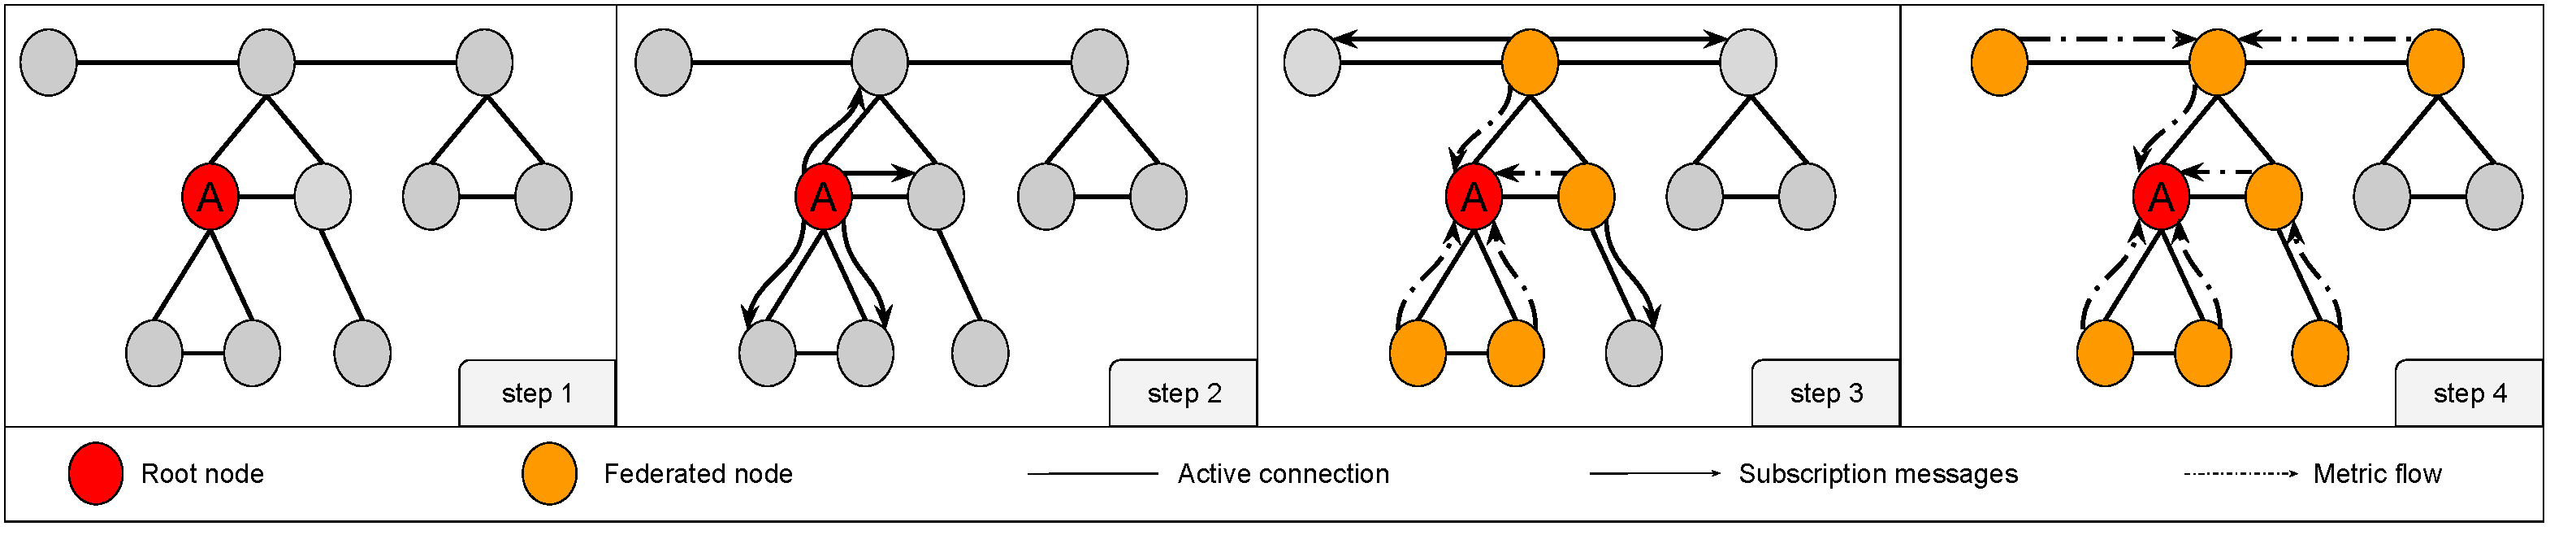
\includegraphics[width=\textwidth]{Chapters/aggregation/images/neigh-agg-subscribe.pdf}
    \caption{Neighborhood aggregation subscription process (TTL=2)}
    \label{fig:mon_protocol:img:neigh_agg_sub}
\end{figure}
     
Whenever a node receives this ``Subscription'' message, it performs the following steps:

\begin{enumerate} \label{sec:mon_protocol:enum:neigh_agg_sub_opts}
    \item Verifies the message came from a node contained in the active view, if it did not, the message is discarded.
    \item Stores, for that sender, the ID of the tree, the TTL of the message and a timestamp of the current time. If there is already such an entry, instead, its timestamp is refreshed.
    \item Decreases the TTL of the message by one.
    \item If the message TTL is 0, the node returns from the procedure.
    \item Following, the node performs the following steps to decide where to broadcast to:
            \begin{enumerate}
                \item If the message came from a parent or a sibling, the node broadcasts the message to its children.
                \item If it came from a child, then the node broadcasts the message to the parent and siblings.
                \item Before broadcasting to any node, the sender verifies if it has sent a ``Subscription'' message with a higher or equal TTL than the TTL from the received one to these nodes in the last (configurable) time window. If it has, the sender skips the message emission for that node.
            \end{enumerate}
\end{enumerate}

With this, in case two different nodes in the system are collecting the same metrics and using the same periodicity, the ``Subscription'' messages are not sent unnecessarily to nodes already subscribed to that tree, because whenever the second ``Subscription'' message arrives, it is not broadcasted unless a certain amount of time has passed. This process is illustrated by node ``A'' in figure \ref{fig:mon_protocol:img:neigh_agg_second_sub}, where it receives the Subscribe message and does not propagate it to its siblings nor parent, as it is already federated to the tree (rooted on itself with TTL= 2) and has sent a ``Subscription'' message to its siblings and parent in the previous step.

\begin{figure}[htbp]
    \centering
    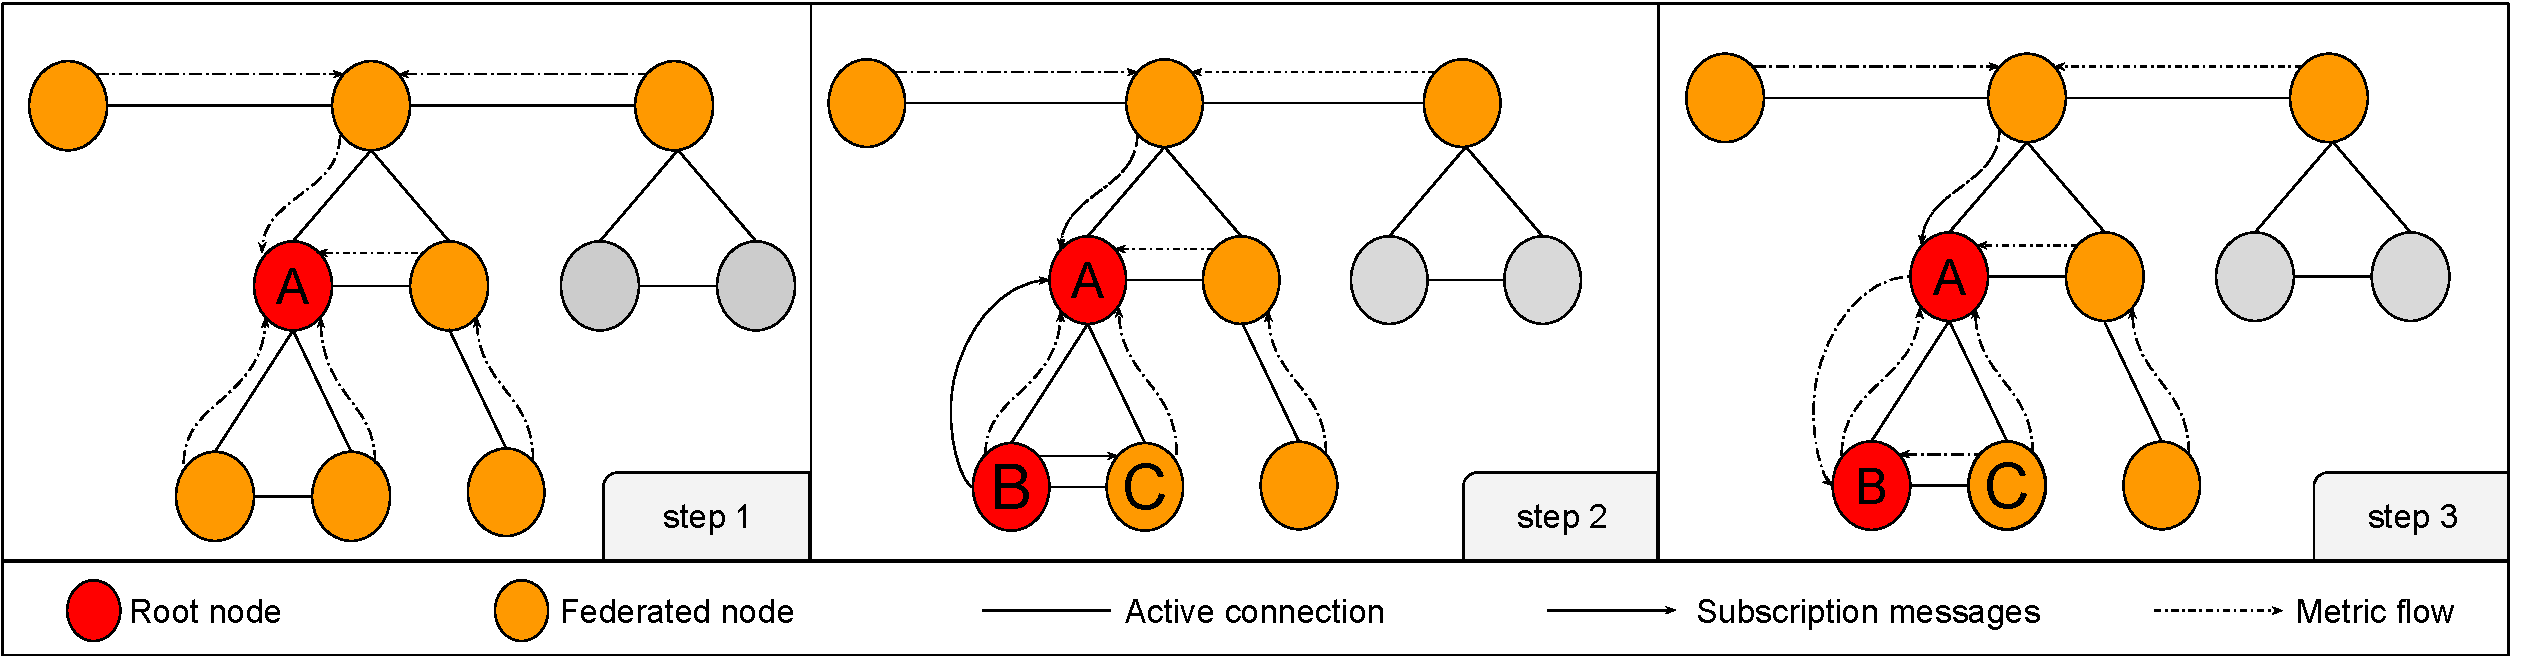
\includegraphics[width=\textwidth]{Chapters/aggregation/images/2nd_subscribe.pdf}
    \caption{Neighborhood aggregation second subscribe (TTL=2)}
    \label{fig:mon_protocol:img:neigh_agg_second_sub}
\end{figure}


\begin{figure}[htbp]
    \centering
    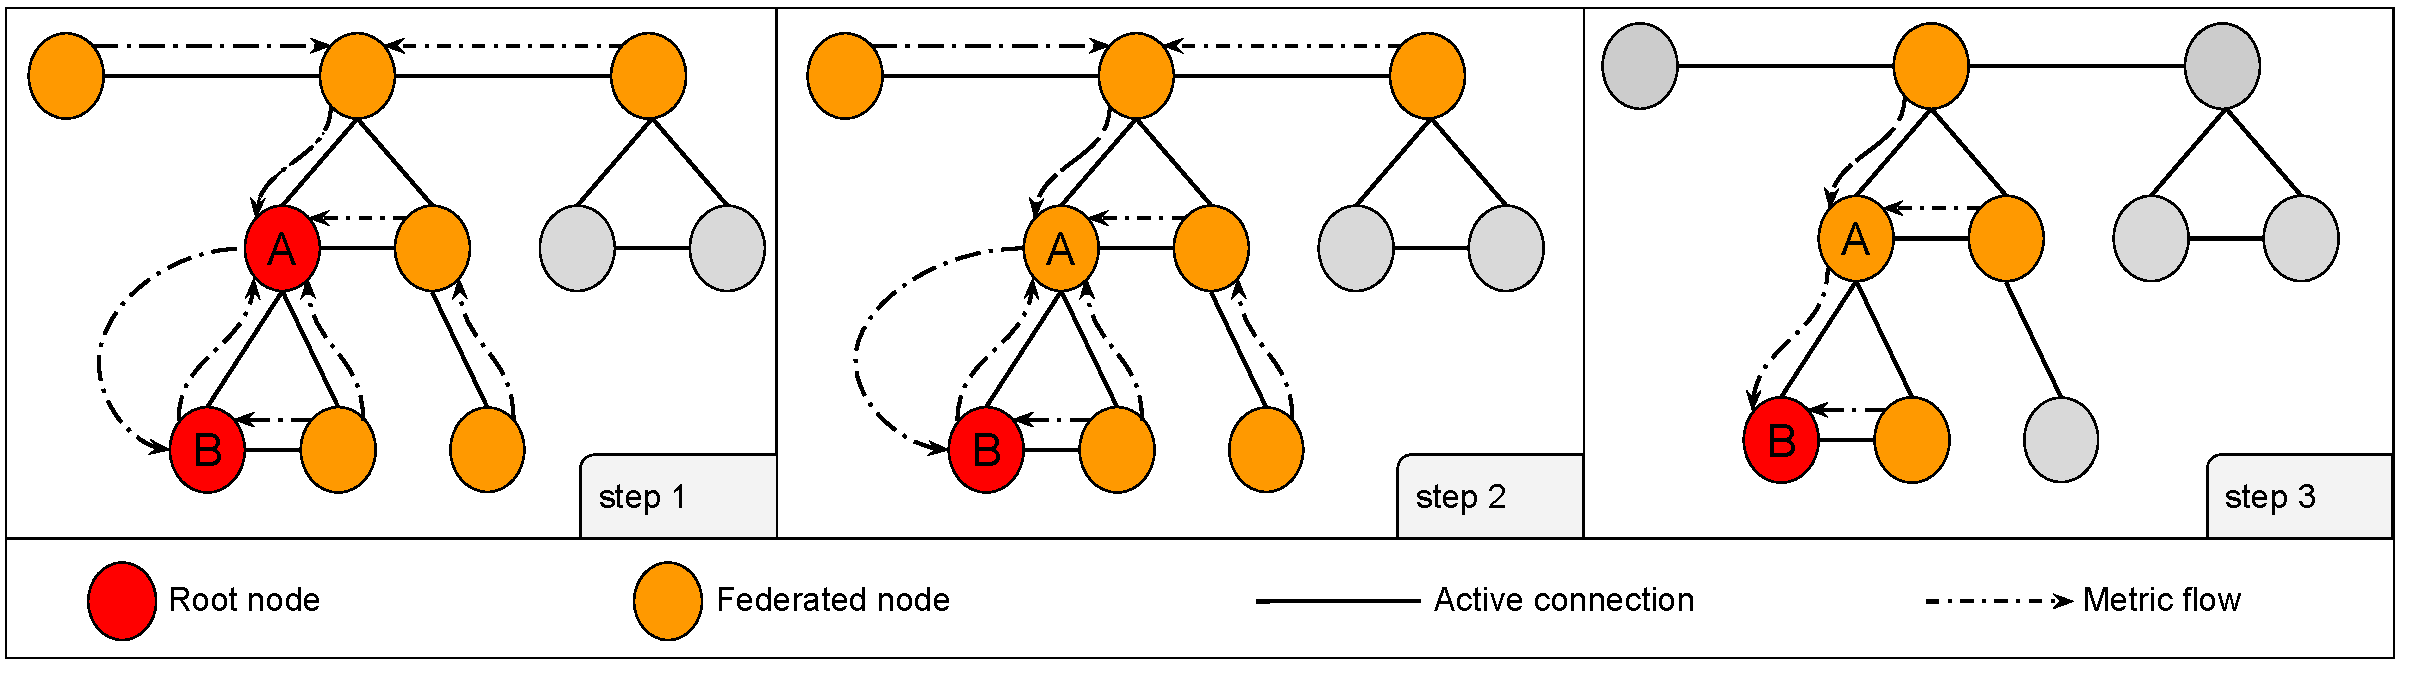
\includegraphics[width=\textwidth]{Chapters/aggregation/images/unsubscribe_process.pdf}
    \caption{Neighborhood unsubscribe (TTL=2)}
    \label{fig:mon_protocol:img:neigh_agg_unsub}
\end{figure}

After nodes become federated in the trees, they begin to periodically evaluate the supplied query and obtain their local metric values (storing them locally if they are a root of that tree). When a node obtains its local metric value, it propagates a message containing the metric value and a hop counter to every other node in its active view that has sent a ``Subscription'' message within a configurable time frame with a TTL lower or equal than the messages'. Nodes that receive the propagation of these values increase the hop counter and repeat this process. This process is illustrated on pictures \ref{fig:mon_protocol:img:neigh_agg_sub} \ref{fig:mon_protocol:img:neigh_agg_second_sub} and \ref{fig:mon_protocol:img:neigh_agg_unsub}). 
    
Lastly, nodes periodically verify, for each tree, the time passed since the reception of the last ``Subscribe'' message. If it exceeds a configurable time frame, the entry is removed, and that node will stop receiving the propagation of metric values. When nodes remove the expired entry, if there is no other entry for that tree ID and the node is not a root of that tree, they delete all metadata related to that tree and stop propagating metric values (illustrated in fig. \ref{fig:mon_protocol:img:neigh_agg_unsub}).

\subsection{Global aggregation} \label{sec:mon_protocol:global_agg}

Global aggregation is the mechanism executed whenever a certain client wishes to obtain a summarized global view of the system (e.g. the total number of nodes in the system). This process, similarly to \ref{sec:mon_protocol:tree_agg} and \ref{sec:mon_protocol:neigh_agg}, is started via a request from the API and functions by federating nodes of the system into \textbf{aggregation trees}, rooted on the nodes that are collecting the aggregate values. In global aggregation, all nodes participate in all aggregation trees, either as a root (if they wish to collect the globally aggregated value), or alternatively as aggregator nodes. Additionally, if a tree has multiple root nodes, then nodes, when possible, reuse the metric values from the first tree root towards the other roots, and deduplicate the maintenance mechanisms of the aggregator trees. 

This mechanism is inspired in the work from Mirage \cite{akosThesis}, which employs an aggregation technique that leverages a tree-shaped overlay to allow the computation of a globally aggregated value in a decentralized and efficient manner by every node in the system. This is achieved via every node periodically broadcasting to every neighbouring peer their aggregated value minus the neighbours' contribution. Nodes that receive this broadcast merge all received contributions with the locally generated one. The continuous execution of this procedure results in all nodes obtaining the global aggregated value without resorting to aggregating the values toward a single node in the system.

% Nodes federated in these trees that are not the roots are denoted \textbf{aggregator} nodes, and their role within this mechanism is to collect their neighbours' metric values, aggregate them, and send them toward the root of the tree.

In this mechanism, we leverage the same aggregation technique to collect globally aggregated values in multiple (but not necessarily all) nodes of the system in a decentralized manner. However, unlike the original work, instead of only performing aggregation of a single metric value, we generalize the approach to allow the on-demand creation and teardown of aggregation trees, rooted in one or more nodes, with all roots collecting the globally aggregated value in a decentralized manner. The relaxation of these constraints creates additional challenges regarding the transmission of redundant messages to maintain the multiple aggregation trees and the decommissioning of the trees, which we attempt to solve in this work. It is important to mention that, in a scenario where all nodes of the system are roots of the aggregation tree, this mechanism behaves similarly to \cite{akosThesis}, with the only difference being of allowing the on-demand start and decommission of the aggregation process.

\begin{algorithm}
    \caption{Global aggregation} \label{alg:mon:global_agg}
    \begin{algorithmic}[1]

    \asdstate \label{alg:mon:global_agg:state_start}
        \State parent : Node \Comment{Defined by the overlay protocol} 
        \State children : dict<string,Node> \Comment{Defined by the overlay protocol} 
        \State siblings : dict<string,Node> \Comment{Defined by the overlay protocol}  
        \State lastTimeSent : dict<string, dict<string, timeStamp>> \asdassign dict()
        \State neighValues : dict<string, dict<value, timeStamp>> \asdassign dict() \label{alg:mon:global_agg:state_end}
        \State tIds : dict<string, <string, string, timeDuration, string, string, boolean, dict< string, timeStamp>> \asdassign dict()
    \asdend

    \asdupon[StartGlobalAggregationRequest(diffF, mergeF, query, periodicity ,outmName)] 
    \label{alg:mon:global_agg:start_req}
        \State tId \asdassign hash(diffF + mergeF + query + periodicity) 
        \If{tId in tIds} 
            \State <diffF, mergeF, query, periodicity, outmName, timerId, isLocal, aggNeighs> \asdassign tIds[tId]
            \State tIds[tId] \asdassign <mergeF, query, periodicity, outmName, timerId, true, aggNeighs>
        \Else
            \State timerID \asdassign registerPeriodicTimer(ExportGlobalAggTimer(tId), periodicity)
            \State tIds[tId] \asdassign <mergeF, query, periodicity, outmName, timerId, true, dict()>
            \State neighValues[tId] = dict()
            \State
        \EndIf
    \asdend

    \asdrepeateveryx{config.PropagateGAggTimeout seconds} \label{alg:mon:global_agg:propag}
        \State toSendArr \asdassign set \label{alg:mon:global_agg:propag_start}
        \For{tId in tIds}
            \State <diffF, mergeF, query, periodicity, outmName, timerId, isLocal, aggNeighs> \asdassign tIds[tId]
            \For{<node, timestamp> in aggNeighs}
                \If{timeSince(timestamp) > config.SubExpirationDuration}
                    \State aggNeighs.remove(node)
                \EndIf
            \EndFor
            \If{aggNeighs.length == 0 \&\& !isLocal}
                \State tIds.remove(tId)
                \State continue
            \EndIf
            \If{isLocal}
                \State toSendArr \asdassign toSendArr + <diffF, mergeF, query, periodicity, outmName, tId>
            \EndIf
        \EndFor
        \State PropagateGAggTrees(toSendArr, parent + children) \label{alg:mon:global_agg:propag_end}
    \asdend

    \asdupon[receive(RefreshGaggTree<gAggs>, sender)] \label{alg:mon:global_agg:propag_recv}
        \State gAggTreeArr \asdassign set 
        \For{<diffF, mergeF, query, periodicity, outmName, tId> in gAggs}
            \If{id in tIds} \label{alg:mon:global_agg:propag_recv_merge}
                \State gAggTreeArr.append(<diffF, mergeF, query, periodicity ,outmName, timerId, tId>)
                \State neighValues[tId] = dict()
                \State tIds[tId] \asdassign <diffF, mergeF, query, periodicity ,outmName, timerId, false, <sender: time.Now()>>
                \State registerPeriodicTimer(HandleTreeAggTimer(tId), periodicity)
            \Else \label{alg:mon:global_agg:propag_recv_merge_end}
                \State <diffF, mergeF, query, periodicity ,outmName, timerId, isLocal, aggNeighs> \asdassign tIds[tId]
                \State aggNeighs[sender] \asdassign time.Now()
                \State tIds[tId] \asdassign <diffF, mergeF, query, periodicity ,outmName, timerId, isLocal, aggNeighs>
                \If{isLocal}
                    \State continue
                \EndIf
            \EndIf
        \EndFor
        \If{sender == parent}
            \State PropagateGAggTrees(gAggTreeArr, children)
        \EndIf
        \If{sender in children}
            \State PropagateGAggTrees(gAggTreeArr, children - sender + parent)
        \EndIf
    \asdend


    \asdupon[ExportGlobalAggTimer(tId)] \label{alg:mon:global_agg:export_trigger}
        \State <diffF, mergeF, query, periodicity, outmName, timerId, isLocal, aggNeighs> \asdassign tIds[tId] \label{alg:mon:global_agg:export_trigger_init_part}
        \State removeOldNeighValues(neighValues[tId])
        \State localVal \asdassign resolveQuery(query)
        \State res \asdassign evalFunc(mergeF, localVal, neighValues[tId])
        \If{isLocal}
            \State storeValLocally(res, outmName)
        \EndIf  \label{alg:mon:global_agg:export_trigger_init_part_end}
        \For{<node, timestamp> in aggNeighs}\label{alg:mon:global_agg:export_trigger_last_part}
            \State sendMessage(PropagateGAggValues<tId, evalFunc(diffF, res, neighValues[tId][node]>, node)
           
        \EndFor \label{alg:mon:global_agg:export_trigger_last_part_end}
    \asdend

    \asdupon[receive(PropagateGAggValues<tId, res>, sender)] \label{alg:mon:global_agg:recv_propag_vals}
        \If{tId in tIds and sender in children || sender == parent}
            \State neighValues[tId][sender] = res, time.Now()
        \EndIf
    \asdend

    \asdprocedure{PropagateGAggTrees(gAggTreeArr, nodeList)} \label{alg:mon:global_agg:propag_procedure}
        \For{node in nodeList}
            \State toSendToNode \asdassign set()
            \For{<diffF, mergeF, query, periodicity ,outmName, timerId, tId> in gAggTreeArr}
                \If{lastTimeSent[node][tId] == nil || time.Since(lastTimeSent[node][tId]) > config.RefreshMessageBackoff}
                    \State toSendToNode \asdassign toSendToNode + <diffF, mergeF, query, periodicity ,outmName, timerId, tId>
                \EndIf
            \EndFor
            \State lastTimeSent[node][tId] \asdassign time.Now()
            \State sendMessage(RefreshGaggTree<toSendToNode>,node)
        \EndFor
    \asdend

    \end{algorithmic}
\end{algorithm}
    

The state necessary for the execution of this mechanism (defined in alg. \ref{alg:mon:global_agg} lines \ref{alg:mon:global_agg:state_start} to \ref{alg:mon:global_agg:state_end}) starts with the active view of the node executing the mechanism, composed by the parent, children and siblings of the node in question. Changes in this view are propagated by notifications emitted by the overlay protocol (these are omitted from the pseudocode). In addition, the state contains a map denominated ``lastTimeSent'', that contains for each tree ID and for each neighbouring node a timestamp, corresponding to the last time that node has refreshed the existence of the tree with that ID. Additionally, each node also maintains a ``neighValues'' map, which stores, for each tree, the propagated neighbour values and a timestamp of the reception of these values. Finally, each node owns a map denominated ``tIds'',  which holds the metadata needed to manage the aggregation trees, composed by: (1) a difference function, used to remove the contributions of a certain node from an aggregated value, (2) the merge function, used for merging two or more values into an aggregated value, (3) the query to obtain the local values, (4) the resulting output name for the aggregated metric, (5) the periodicity at which to collect the aggregated value, (6) a boolean representing if the node executing the protocol is a root of the aggregation tree, and finally, (7) a map called ``aggNeighs'' which contains the peers that are interested in receiving values for that tree (previously referred to as the aggregator nodes).

This mechanism is initiated with the reception of a request from the API (line \ref{alg:mon:global_agg:start_req}), which contains multiple parameters: (1) the difference function, (2) the merge function, (3) the query to obtain the local value (4) the periodicity to perform this mechanism, and (5) the resulting metric name (to label the output values). Upon reception of this request, the node hashes the concatenation of the difference function, the merge function, the query, and the periodicity of the request, obtaining the tree ID, which will be common to every node in the tree. After the ID generation, the node checks if there already is a tree with that ID present in its local ``tIds'' map, setting as true the variable which denotes if the node should save the aggregated value locally. If there is no tree with such ID previously present, the node sets up a new ``ExportGlobalAggTimer'' with the provided periodicity and creates a new entry in the ``neighValues'' map for that tree.

As previously mentioned, global aggregation allows the on-demand creation and decommission of aggregation trees. This process is defined in alg. \ref{alg:mon:global_agg} lines \ref{alg:mon:global_agg:propag_start} to \ref{alg:mon:global_agg:propag_end}), where, as previously mentioned, nodes periodically send messages named ``RefreshGaggTree'' containing the aggregation trees they are the roots of to their children and parent and clear all entries in the ``aggNeighs'' that are older than a configured time frame. If a tree has no more entries in this map, and the ``isLocal'' flag is not set to true, then that tree is decommissioned.

% This process is achieved through a time-based mechanism, where nodes periodically refresh the trees they are the roots of via message broadcasts which are then forwarded by other nodes in the system until they reach every node. If an aggregator node (not a root) does not receive a message from any neighbour refreshing the existence of a tree within a certain time frame, it decommissions the tree locally. 

Whenever the ``RefreshGaggTree'' message is received (alg. \ref{alg:mon:global_agg} line \ref{alg:mon:global_agg:propag_recv}), the receiver adds the previously unknown trees into its local ``tIds'' map and sets up a periodic ``ExportGlobalAggTimer'' for each added tree (lines \ref{alg:mon:global_agg:propag_recv_merge} to \ref{alg:mon:global_agg:propag_recv_merge_end}). Alternatively, if the tree was previously in the ``tIds'' map, the node refreshes the sender's entry in the ``aggNeighs'' map. Finally, the node removes the trees present in the message where it is also a root of (deduplicating the tree maintenance mechanisms) and forwards the remaining trees to every node in its active view, excluding the sender. Before transmitting the trees to each node, the node checks, for each tree, if it has transmitted a ``RefreshGaggTree'' message containing the same tree in the last (configurable) time frame. If it has, then it does not propagate that tree to that node. These verifications are performed to prevent trees from being refreshed multiple times unnecessarily. 

\subsubsection{Metric propagation}

With the aggregation tree established, we now explain how the values are propagated and aggregated by each tree in the system. As previously mentioned, nodes set up an ``ExportGlobalAggTimer'' for each registered tree, whenever this timer triggers (alg.  \ref{alg:mon:global_agg} line \ref{alg:mon:global_agg:export_trigger}), the node first removes all out-of-date neighbour values for the corresponding tree (according to a configurable timeout) and evaluates the query, obtaining its local value. Then, using the neighbour values and the locally obtained value, it applies the merge function and obtains the globally aggregated value, which it stores locally if configured by the ``isLocal'' flag (lines \ref{alg:mon:global_agg:export_trigger_init_part} to \ref{alg:mon:global_agg:export_trigger_init_part_end}). Then, for each entry previously in the ``aggNeighs'' map, it sends a ``PropagateGAggValues'' message with the aggregated value minus the node's contribution and the tree ID. (lines \ref{alg:mon:global_agg:export_trigger_last_part} to \ref{alg:mon:global_agg:export_trigger_last_part_end}). 

Finally, whenever nodes receive the ``PropagateGAggValues'' message (alg. \ref{alg:mon:global_agg} line \ref{alg:mon:global_agg:export_trigger}) containing the aggregated value and the tree ID, they verify that it was sent from either the parent or the children and that the tree ID is in their local ``tIds'' map, discarding the message any one of these conditions is observed. Finally, they store the propagated value locally in their ``neighValues'' map for later use in computing the aggregated value.

In sum, nodes that are roots of their aggregation trees will, over time, receive aggregated values from their nodes, which are essentially sent and aggregated by all other nodes using the reverse path taken by the``RefreshGaggTree'' messages. Given the fact that nodes only use their parents and children of the tree topology to forward messages (thus ensuring the tree has no cycles, as there is only a single path from any node to each other node in the system), by propagating to a neighbour the resulting aggregated value without the effects of its contribution \cite{akosThesis}, multiple nodes in the system can simultaneously obtain the aggregated value efficiently and in a decentralized manner.

\subsection{Summary}

In this section, we presented the devised aggregation protocol. This protocol leverages the devised overlay protocol's tree structure to perform efficient propagation/aggregation of information in a decentralized manner. This protocol is coalesced by three decentralized information aggregation/collection primitives, which we believe to be useful for gathering partial or complete system information to perform decentralized resource management actions. 

The first primitive is \textbf{tree aggregation}, where nodes, when requested, form aggregation trees (with configurable range) rooted upon themselves. These trees extend only to their descendants in the original overlay protocol tree, and nodes federated in these trees periodically merge their local value with their childrens' and send a message containing it to their parent. In case one descendant is executing the same primitive with a tree with the same range (from the descendants' perspective), it simply reuses the parent's tree to obtain the intended aggregated value. 

The second primitive is \textbf{neighborhood aggregation}, where nodes collect, on-demand and in a decentralized manner, the metrics of nodes in a hop-defined range. This mechanism behaves similarly to a pub-sub system, where nodes periodically propagate messages which federate other nodes in trees rooted upon themselves. Nodes in these trees propagate their local values periodically using the reverse paths taken by the federation messages. In this primitive, nodes (when possible) deduplicate federation messages and multiplex metric propagations.

Lastly, the third primitive called \textbf{global aggregation} is a primitive where nodes collect and aggregate, also on-demand and in a decentralized manner, a value that corresponds to the globally aggregated value of the system. This primitive is inspired by work from the state-of-the-art, however, it relaxes constraints imposed by the original work, such as performing the mechanism with only a partial set of the nodes being tree roots, in addition to allowing the technique to be performed in an on-demand fashion (based on API requests).

We believe these primitives are useful for resource management decisions such as, for example, maintaining a proportion of replicas to nodes, by employing \textbf{tree aggregation} collecting all the descendants' number of replicas and number of nodes, the tree roots can, in a decentralized and independent manner, perform replication or decommission of replicas to maintain the target value. The same applies to \textbf{global aggregation}, which allows nodes to, for example, collect the total number of replicas in the system and perform replication actions if they reach a lower than configured number. Lastly, \textbf{neighbourhood aggregation} allows nodes to collect information about nearby nodes, which can also be used to improve system QOS by, for example, deploying a server closer to a client in terms of geographical distance.

It is important to mention that while in this work we present the protocol leveraging the overlay protocol defined in \ref{sec:overlay_network}, the protocol is agnostic to which overlay protocol is executing underneath it, as long as it has the following characteristics: (1) forms one or more tree-shaped networks, whose roots are interconnected; (2) Nodes in these trees must be connected to their parents, children and siblings (also denoted by their active view) with bidirectional connections; and finally (3) the overlay protocol must also provide events for each node that is added or removed from the protocols' active view.

% As previously mentioned in \ref{sec:mon_protocol}
% 
As previously mentioned, these decentralized aggregation primitives make use of both queries and aggregation functions to obtain the data and to summarize it (respectively). In this next section, we cover the monitoring module that, along with other features, interprets and processes the aforementioned queries and aggregation functions.

\section{Monitoring module}
\label{sec:mon_module}


The \textbf{monitoring module} is tasked with storing metrics, resolving queries regarding stored metrics, removing expired metrics, periodically evaluating registered alarms, triggering callbacks which the API then propagates to the client, among other features which we will now cover.

We believe it is, however, important to remember that the focus of this work is to provide a usable proof-of-concept of a decentralized monitoring framework, targeted for decentralized resource management solutions. Consequently, the focus of this module is to provide just enough functionality for a proof of concept, namely in aspects such as the storage of metrics in disk or the efficiency of the query language, which are interesting research challenges by themselves, however are orthogonal to the conducted work. 

This module is composed by three different components (illustrated by fig. \ref{fig:mon_module_overview}): the \textbf{query engine}, the \textbf{time-series database} (TSDB)), and the \textbf{alert manager}, whose roles in the system we now briefly explain:

\begin{figure}[htbp]
    \centering
    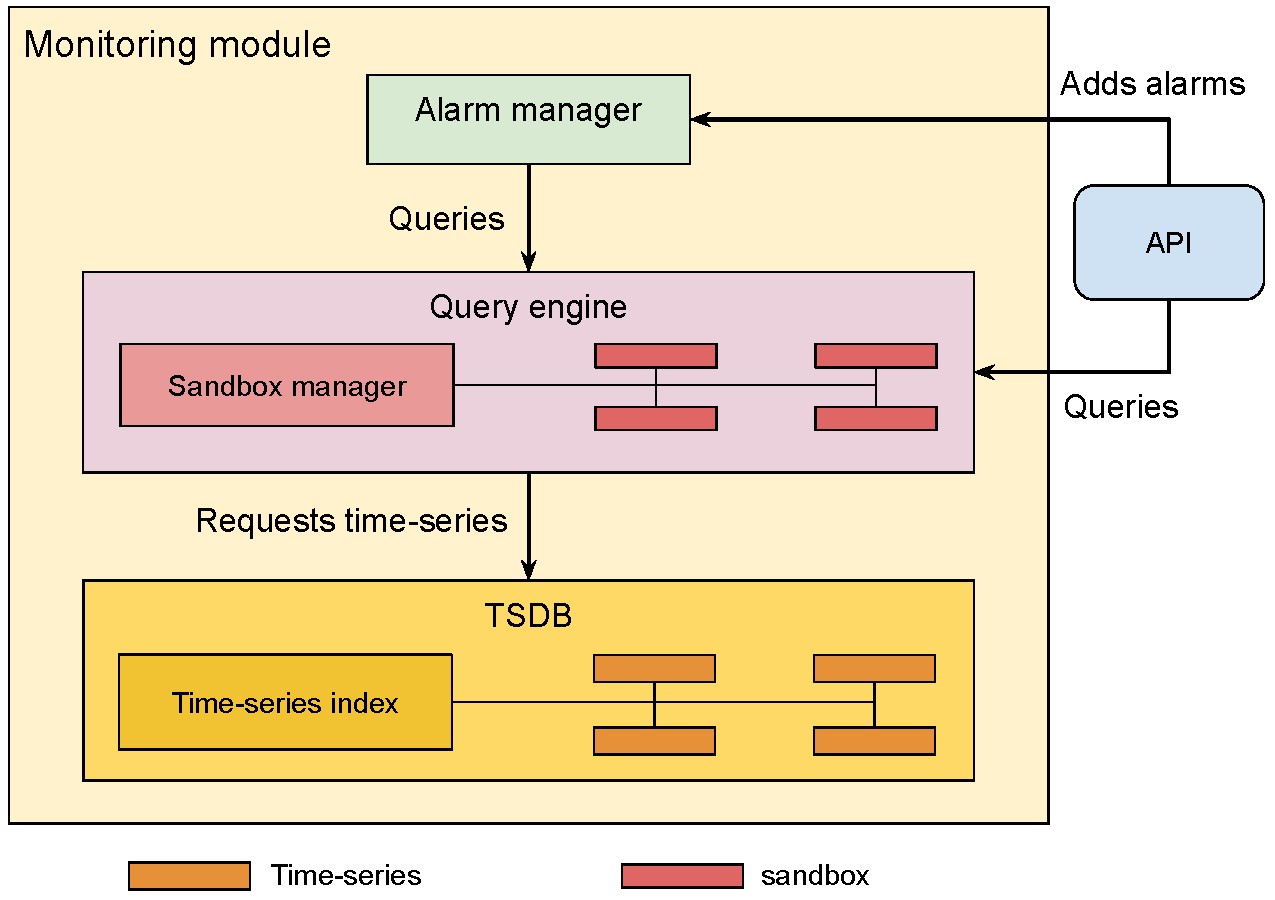
\includegraphics[width=\textwidth]{Chapters/mon_module/images/Monitoring_module.pdf}
    \caption{An overview of the monitoring module}
    \label{fig:mon_module_overview}
\end{figure}

\begin{enumerate}
    
    \item The \textbf{time-series database} allows the insertion and retrieval of time-series data from the framework. This time-series database employs an in-memory index to retrieve one or more time-series according to a set of parameters.

    \item The \textbf{query engine} is the component tasked with resolving queries made to the time-series database. This component maintains a set of sandboxes that evaluate user-provisioned queries that both extract data from the database and apply aggregation functions to it.
    
    \item Finally, the \textbf{alert manager} manages the alarms issued by the API. In sum, this component periodically verifies the issued alarms' query using the \textbf{query engine} and propagates an event to the client whenever the condition is verified.
     
\end{enumerate}

In order to ease the explanation of these components, we first detail the structure of the metrics used in this framework, which has a similar structure to the metric types provided by InfluxDB \cite{influxdb_data_elements}. 

\subsubsection{Metric  structure}

In DeMMon, a metric is composed of four elements: first, the \textbf{name}, which is a string denoting the name of the stored information, the name should be a human-readable name which is self-describing (e.g. ``CPU-USAGE''). The second element are the metric \textbf{tags}, which are a set of string pairs denoting attributes related to the metric that is stored, (e.g. the hostname or cluster name of the node that emitted it), next, we have the \textbf{value}, which contains the data associated with the observed metric, and finally, we have the  \textbf{timestamp}, that contains the time at which the observation was taken. A typical example of a metric in the devised framework would be: name: ``CPU-Usage''; tags: <host:nodeX>, value: 0.3, timestamp: ``1609960731''.

We believe it is important to mention that in order to remain as flexible as possible, the metric values do not have a defined type. In this system, clients may use custom types (as long as they are serializable using the JSON package provided by the Golang \cite{golang} package). This allows the devised framework to represent a multitude of different information types, such as histograms, strings, string maps, among others, which offers a higher degree of flexibility for using this framework. For example, a decentralized service management system aimed at deploying service replicas in close proximity to the clients may use, for example, a histogram with pre-determined geographical classes. This way, this system would have a data structure that would ease finding a node in the desired geographical area.

Provided with the metric structure, we now explain how these are stored in the system. 

\subsubsection{Time-series database}  \label{sec:mon_module:tsdb}

In DeMMon, time-series are sequences taken at successive equally spaced points in time. In this system, time-series are stored only in memory and are indexed as a function of their name and tags.

In order for a certain metric (composed by: name, tags, and periodicity) to be inserted into the database, a \textbf{bucket} must first be created. A bucket is essentially a component that holds all time-series data with a certain name, periodicity and capacity. The periodicity denotes the interval at which the sequences of points are spaced (in time) and the capacity denotes the number of points stored in each sequence. For example, a time-series with a 5-second periodicity and a capacity of 12 holds all points from the last minute. Limiting the number of points per series allows the system to pre-allocate the memory necessary (using an array) for each time-series at the time of its creation.

Within a bucket, metrics are stored in a map and indexed by their tags. This is done by generating keys that are equal for each similar tag set, independent of its order: whenever a metric is inserted, the tag pairs are sorted alphabetically (by their key) and concatenated into a single string, producing the resulting metric key. Then, using the metric key, the metric value is inserted into the corresponding time-series (a new time-series is created for that tag set if there was none previously in the system).

Time-series advance time in an on-demand manner, meaning that, before returning values for any read or write request from a time-series, the system first verifies if its' oldest value has a timestamp outside of the time-series window (as time has passed since the last check). If it has, the system iterates the time-series' points from its oldest to the newest point and removes all points outside its time window. In order to remove unused time-series from the system, and decrease DeMMons' memory footprint, the time-series database component also periodically advances the time-series in time and removes any that become empty.

Concurrency is maintained using locking mechanisms, where operations that do not affect the state of the time-series are executed concurrently, and operations that would otherwise change the time-series status are executed sequentially. 



\subsubsection{Query engine} \label{sec:mon_module:query_engine}

The query engine is a sub-component of the monitoring module, and it is responsible for evaluating the supplied text-based queries, transforming them into sets of instructions, and determining the final query result by executing the instructions. Keeping in mind the fact that the focus of this work is not the performance of the metric storage or the query language and that it is still a focal point of this work to be as flexible as possible in the query language, we opted for using javascript-based sandboxes to perform this work. This means that user-provided queries are essentially javascript code, and consequently, users have infinite control over the behaviour of their queries, provided these do not exceed the query timeout.

In order to provide this functionality, we opted for using the package Otto \cite{otto}. This package provides access to javascript ``virtual machines'' that essentially parse a string containing javascript code, and produce an AST from the parsed code. The produced ASTs are then executed and their result is returned by the VM. In order to allow users to access the time-series stored in the TSDB , the query engine provides every Otto virtual machine access to the following functions, which return time-series from the database:

\begin{enumerate}

    \item Select(Bucket\_Name, <Tag\_set\_regex), this function returns the time-series that are in the supplied bucket matching the provided tag set regex. The way the tag set regex matching works is: for every time series present in the specified bucket, if all of the tag keys in the supplied regex match all of the time series tags, then the time series is returned. An example of the usage of this function would be, for example: ``select(CPU\_USAGE, <host:.*, cluster:cluster1>)''

    \item SelectLast(Bucket\_Name, <Tag\_set\_regex>), this function behaves similarly to Select, however, it only returns the last inserted point in all matched time series.
    
    \item SelectRange(Bucket\_Name, <Tag\_set\_regex>, startDate, endDate), this function behaves similarly to ``Select'' and ``SelectLast'', however, it allows users to only extract a certain time-window from the matching time-series. To do so, it takes an additional argument, consisting of a time range, used to filter the points to return to the client.
    
\end{enumerate}

% With these three functions, clients can select either partial sets of points or the totality of points from every time series stored in the database, which are then usable in the javascript code.  

We believe these functions cover the most common use cases for metric selection. These metrics, upon selection, can then be aggregated in any way the user specifies in the query (since they are composed of user-defined code). In order to ease the design of queries and prevent developers from rewriting the same aggregation functions, the query engine also provides some aggregation primitives which can be applied to one or more time-series such as: Max, Min and Average.

After the selection and aggregation of metrics, the resulting values are returned by placing them in a variable denoted ``result'' (in the user-defined code). Any query executed in DeMMon can only result in one of two types: a single time series or an array of time series (following an interface defined by DeMMon). Given this, in order to allow the creation of new time series that follow this interface during the query process, there are two additional functions supplied to the virtual machines: the first is called ``NewTimeSeries'', which creates a new time series, this function takes as arguments the name, tags and values which will integrate the time series; second, we have the function called ``NewObservable'' which takes a value of any type and a timestamp, and creates a new metric point which can be added to time series.

 With this, we now provide some examples of possible queries along with a brief description of what they do:

\begin{enumerate}
    \item ``Avg(SelectLast(CPU\_USAGE, <host:.*, cluster:cluster1>))'' this query selects the metrics with the name ``CPU\_USAGE'' for all hosts which belong to cluster with name ``cluster1'' and returns the average of all the points.
    
    \item ``SelectLast(Nr\_services, <tenant:tenant10>, startDate, endDate)'' this query returns the timeseries for the metric called ``Nr\_services'' for the tenant with name ``tentant10'' during the provided time range.

    \item ``SelectLast(Nr\_replicas, <tenant:tenant10,service:service10>)'' this query returns the timeseries for the metric called ``Nr\_replicas'' for the tenant with name ``tentant10'' and service named ``service10'' during the provided time range.
    
    % \item \todo{meter mais um exemplo de uma query custom}
    
\end{enumerate}

With this, clients are able to obtain and manipulate data from the time series database using text-based queries. Furthermore, as the type of the value of each metric is not enforced, clients may store their metrics in custom data structures, tailored for their specific use-cases.

\subsubsection{Alarm manager} \label{sec:mon_module:alarm_monitor}

The alert manager is the last component of the monitoring module, it is responsible for managing the \textbf{alarms} issued to the monitoring module. Alarms are essentially sets of parameters that contain, among other parameters, a condition to observe (e.g. the percentage of CPU usage) and a periodicity to observe this condition. Alarms are paramount to prevent applications from having to periodically query DeMMon to verify the condition themselves, effectively saving bandwidth. This component is essentially responsible for periodically verifying these alarms and issuing notifications to the client whenever their conditions are verified. 

In DeMMon, an alarm contains the following parameters: 

\begin{enumerate}
    \item \textbf{Condition}. This is essentially a query (explained in \ref{sec:mon_module:query_engine}) that must return a boolean value.
    
    \item \textbf{Periodicity}. The periodicity denotes how often the condition is evaluated, and how often notifications are sent to the client that issued the alarm
    
    \item \textbf{Backoff time}. The backoff time is a time duration that bounds the rate at which the monitoring module emits notifications, which would otherwise happen at the alarm periodicity every time the alarm is verified (e.g. if the supplied periodicity is low).
    
    \item \textbf{Watch list}. The watch list is a set that, for every item, contains both a name and a set of tag filters. Whenever the alarm manager receives an alarm containing a watch list, in addition to performing the verification at the specified periodicity, it also performs the verification whenever any time series matching the watch list is changed. The rates at which the alarm is verified in this manner also respects the backoff time.
    
    \item \textbf{CheckPeriodic}. CheckPeriodic is a boolean variable denoting if the alarm should be verified periodically. When false, the alarm manager does not check the metrics at every \textbf{``periodicity''} seconds (defined previously), effectively saving CPU time. This option is meant to be used together with the watch list, for example, for checking a parameter that is rarely altered.
    
\end{enumerate}

The monitoring module, whenever it receives a new alarm, essentially adds it to a priority queue containing all the alarms. This priority queue uses the time of reception of the alarms plus their periodicity as their key to the queue. With this, alarms are sorted by the time at which they need to be verified. The monitoring module continuously obtains and removes the first item of the queue, containing the next alarm to verify out of all issued alarms and waits until it is time of verification of that alarm (i.e. the time of reception of the alarm plus its periodicity). Ater this, it evaluates the condition (emitting a notification to the client if the condition is verified), and re-adds the alarm to the queue with a key corresponding to the current time plus the alarms' periodicity. Whenever an alarm is verified, and the result of its condition returns ``true'', the alarm manager first verifies if it has emitted a notification for that alarm in the last ``Backoff time'' duration, and issues a notification to the client if it has not.

\section{API}
\label{sec:api}

\subsection{Overview}



\section{Summary}

In this chapter, we covered the implementation of the DeMMon framework, a decentralized management and monitoring framework targeted for the operation of decentralized resource management systems. We began by covering what we believe to be the requirements of this solution (enum. \ref{enum:demmon}). Following, we provided a brief overview of the four modules which compose this framework, beginning with the overlay network (sec. \ref{sec:overlay_network}), which is responsible for creating and maintaining a multi-tree shaped network, optimized using latencies and node capacity. Following, in Section \ref{sec:mon_protocol} we covered the aggregation protocol, which provides multiple primitives for collecting and aggregating metrics in a decentralized and efficient manner, using in-transit aggregation, from a partial (or complete) set of nodes in the tree-shaped network. Next, we covered the monitoring module (sec. \ref{sec:mon_module}), which is the module responsible for enabling the storage and retrieval of metrics, parsing and processing queries and managing alarm lifecycles. Finally, we finished the DeMMon implementation by covering the API (sec. \ref{sec:api}), which essentially is the module responsible for mediating, via a WebSockets interface, the aforementioned interactions between the external clients and the other modules.